\documentclass[11pt,]{article}
\usepackage[left=1in,top=1in,right=1in,bottom=1in]{geometry}
\newcommand*{\authorfont}{\fontfamily{phv}\selectfont}
\usepackage[]{mathpazo}


  \usepackage[T1]{fontenc}
  \usepackage[utf8]{inputenc}



\usepackage{abstract}
\renewcommand{\abstractname}{}    % clear the title
\renewcommand{\absnamepos}{empty} % originally center

\renewenvironment{abstract}
 {{%
    \setlength{\leftmargin}{0mm}
    \setlength{\rightmargin}{\leftmargin}%
  }%
  \relax}
 {\endlist}

\makeatletter
\def\@maketitle{%
  \newpage
%  \null
%  \vskip 2em%
%  \begin{center}%
  \let \footnote \thanks
    {\fontsize{18}{20}\selectfont\raggedright  \setlength{\parindent}{0pt} \@title \par}%
}
%\fi
\makeatother




\setcounter{secnumdepth}{3}

\usepackage{color}
\usepackage{fancyvrb}
\newcommand{\VerbBar}{|}
\newcommand{\VERB}{\Verb[commandchars=\\\{\}]}
\DefineVerbatimEnvironment{Highlighting}{Verbatim}{commandchars=\\\{\}}
% Add ',fontsize=\small' for more characters per line
\usepackage{framed}
\definecolor{shadecolor}{RGB}{248,248,248}
\newenvironment{Shaded}{\begin{snugshade}}{\end{snugshade}}
\newcommand{\KeywordTok}[1]{\textcolor[rgb]{0.13,0.29,0.53}{\textbf{#1}}}
\newcommand{\DataTypeTok}[1]{\textcolor[rgb]{0.13,0.29,0.53}{#1}}
\newcommand{\DecValTok}[1]{\textcolor[rgb]{0.00,0.00,0.81}{#1}}
\newcommand{\BaseNTok}[1]{\textcolor[rgb]{0.00,0.00,0.81}{#1}}
\newcommand{\FloatTok}[1]{\textcolor[rgb]{0.00,0.00,0.81}{#1}}
\newcommand{\ConstantTok}[1]{\textcolor[rgb]{0.00,0.00,0.00}{#1}}
\newcommand{\CharTok}[1]{\textcolor[rgb]{0.31,0.60,0.02}{#1}}
\newcommand{\SpecialCharTok}[1]{\textcolor[rgb]{0.00,0.00,0.00}{#1}}
\newcommand{\StringTok}[1]{\textcolor[rgb]{0.31,0.60,0.02}{#1}}
\newcommand{\VerbatimStringTok}[1]{\textcolor[rgb]{0.31,0.60,0.02}{#1}}
\newcommand{\SpecialStringTok}[1]{\textcolor[rgb]{0.31,0.60,0.02}{#1}}
\newcommand{\ImportTok}[1]{#1}
\newcommand{\CommentTok}[1]{\textcolor[rgb]{0.56,0.35,0.01}{\textit{#1}}}
\newcommand{\DocumentationTok}[1]{\textcolor[rgb]{0.56,0.35,0.01}{\textbf{\textit{#1}}}}
\newcommand{\AnnotationTok}[1]{\textcolor[rgb]{0.56,0.35,0.01}{\textbf{\textit{#1}}}}
\newcommand{\CommentVarTok}[1]{\textcolor[rgb]{0.56,0.35,0.01}{\textbf{\textit{#1}}}}
\newcommand{\OtherTok}[1]{\textcolor[rgb]{0.56,0.35,0.01}{#1}}
\newcommand{\FunctionTok}[1]{\textcolor[rgb]{0.00,0.00,0.00}{#1}}
\newcommand{\VariableTok}[1]{\textcolor[rgb]{0.00,0.00,0.00}{#1}}
\newcommand{\ControlFlowTok}[1]{\textcolor[rgb]{0.13,0.29,0.53}{\textbf{#1}}}
\newcommand{\OperatorTok}[1]{\textcolor[rgb]{0.81,0.36,0.00}{\textbf{#1}}}
\newcommand{\BuiltInTok}[1]{#1}
\newcommand{\ExtensionTok}[1]{#1}
\newcommand{\PreprocessorTok}[1]{\textcolor[rgb]{0.56,0.35,0.01}{\textit{#1}}}
\newcommand{\AttributeTok}[1]{\textcolor[rgb]{0.77,0.63,0.00}{#1}}
\newcommand{\RegionMarkerTok}[1]{#1}
\newcommand{\InformationTok}[1]{\textcolor[rgb]{0.56,0.35,0.01}{\textbf{\textit{#1}}}}
\newcommand{\WarningTok}[1]{\textcolor[rgb]{0.56,0.35,0.01}{\textbf{\textit{#1}}}}
\newcommand{\AlertTok}[1]{\textcolor[rgb]{0.94,0.16,0.16}{#1}}
\newcommand{\ErrorTok}[1]{\textcolor[rgb]{0.64,0.00,0.00}{\textbf{#1}}}
\newcommand{\NormalTok}[1]{#1}
\usepackage{longtable,booktabs}

\usepackage{graphicx,grffile}
\makeatletter
\def\maxwidth{\ifdim\Gin@nat@width>\linewidth\linewidth\else\Gin@nat@width\fi}
\def\maxheight{\ifdim\Gin@nat@height>\textheight\textheight\else\Gin@nat@height\fi}
\makeatother
% Scale images if necessary, so that they will not overflow the page
% margins by default, and it is still possible to overwrite the defaults
% using explicit options in \includegraphics[width, height, ...]{}
\setkeys{Gin}{width=\maxwidth,height=\maxheight,keepaspectratio}

\title{Características morfométricas de la microcuenca Caña, República
Dominicana, aplicando tecnología geoespacial de código abierto.  }



\author{\Large Cinthia Amalia Vandepool Candelario\vspace{0.05in} \newline\normalsize\emph{Estudiante de Geografía mención Recursos Naturales y Ecoturismo,
Universidad Autónoma de Santo Domingo (UASD)}  }


\date{}

\usepackage{titlesec}

\titleformat*{\section}{\normalsize\bfseries}
\titleformat*{\subsection}{\normalsize\itshape}
\titleformat*{\subsubsection}{\normalsize\itshape}
\titleformat*{\paragraph}{\normalsize\itshape}
\titleformat*{\subparagraph}{\normalsize\itshape}

\titlespacing{\section}
{0pt}{36pt}{0pt}
\titlespacing{\subsection}
{0pt}{36pt}{0pt}
\titlespacing{\subsubsection}
{0pt}{36pt}{0pt}





\newtheorem{hypothesis}{Hypothesis}
\usepackage{setspace}

\makeatletter
\@ifpackageloaded{hyperref}{}{%
\ifxetex
  \PassOptionsToPackage{hyphens}{url}\usepackage[setpagesize=false, % page size defined by xetex
              unicode=false, % unicode breaks when used with xetex
              xetex]{hyperref}
\else
  \PassOptionsToPackage{hyphens}{url}\usepackage[unicode=true]{hyperref}
\fi
}

\@ifpackageloaded{color}{
    \PassOptionsToPackage{usenames,dvipsnames}{color}
}{%
    \usepackage[usenames,dvipsnames]{color}
}
\makeatother
\hypersetup{breaklinks=true,
            bookmarks=true,
            pdfauthor={Cinthia Amalia Vandepool Candelario (Estudiante de Geografía mención Recursos Naturales y Ecoturismo,
Universidad Autónoma de Santo Domingo (UASD))},
             pdfkeywords = {morfometría fluvial, modelo digital de elevación, red de drenaje, razón
de bifurcación, indice de convavidad},  
            pdftitle={Características morfométricas de la microcuenca Caña, República
Dominicana, aplicando tecnología geoespacial de código abierto.},
            colorlinks=true,
            citecolor=blue,
            urlcolor=blue,
            linkcolor=magenta,
            pdfborder={0 0 0}}
\urlstyle{same}  % don't use monospace font for urls

% set default figure placement to htbp
\makeatletter
\def\fps@figure{htbp}
\makeatother

\usepackage{pdflscape} \newcommand{\blandscape}{\begin{landscape}}
\newcommand{\elandscape}{\end{landscape}}


% add tightlist ----------
\providecommand{\tightlist}{%
\setlength{\itemsep}{0pt}\setlength{\parskip}{0pt}}

\begin{document}
	
% \pagenumbering{arabic}% resets `page` counter to 1 
%
% \maketitle

{% \usefont{T1}{pnc}{m}{n}
\setlength{\parindent}{0pt}
\thispagestyle{plain}
{\fontsize{18}{20}\selectfont\raggedright 
\maketitle  % title \par  

}

{
   \vskip 13.5pt\relax \normalsize\fontsize{11}{12} 
\textbf{\authorfont Cinthia Amalia Vandepool Candelario} \hskip 15pt \emph{\small Estudiante de Geografía mención Recursos Naturales y Ecoturismo,
Universidad Autónoma de Santo Domingo (UASD)}   

}

}








\begin{abstract}

    \hbox{\vrule height .2pt width 39.14pc}

    \vskip 8.5pt % \small 

\noindent La morfometría fluvial es de gran importancia para realizar estudios
hidrológicos en un contexto de cambio climático con amenazas cada vez
más frecuentes de eventos extremos, pero aún en la actualidad pocos
países realizan de manera continua análisis de esta índole, en especial
en nuestro país que, debido a su condición como isla y su ubicación en
la trayectoria de ciclones tropicales, debería de estar especialmente
interesado en mitigar el riego de grandes inundaciones. A lo largo de
este artículo se estará analizando la microcuenca del arroyo caña,
perteneciente a la subcuenca del río Macasía ubicada en el extremo
suroeste de la República Dominicana, dicha unidad hidrográfica es
prácticamente desconocida, ya que no se posee información específica
sobre ella en fuentes bibliográficas, por lo que este estudio
proporciona algunos datos reales sobre sus aspectos morfométricos,
geológicos y cartográficos. Basándose en datos preexistentes y
utilizando un MDE se delimitó la cuenca y se analizó la red de drenaje y
los perfiles longitudinales e indices de concavidad del curso más largo,
de la misma forma se calcularon los parámetros morfométricos de la
cuenca, se estudió su posible relación con la litología de la zona y si
existían evidencias de un posible fenómeno de reorganizamiento del
drenaje.


\vskip 8.5pt \noindent \emph{Keywords}: morfometría fluvial, modelo digital de elevación, red de drenaje, razón
de bifurcación, indice de convavidad \par

    \hbox{\vrule height .2pt width 39.14pc}



\end{abstract}


\vskip 6.5pt


\noindent  \section{Introducción}\label{introducciuxf3n}

A lo largo del último siglo se ha reducido la dificultad para realizar
análisis espaciales, gracias a los novedosos avances tecnológicos en el
desarrollo de los Sistemas de Información Geográfica (SIG) se ha
simplificado el arduo trabajo que suponía llevar a cabo este tipo de
análisis, y a pesar de todas las herramientas disponibles, la República
Dominicana aún está pasos por detrás de muchos países en especial en lo
relacionado con los análisis de geomorfología fluvial, situación
lamentable, ya que la isla posee innumerables cursos fluviales
permitiéndole ocupar un lugar privilegiado en este siglo, ya que, cada
día más países sufren por la escasez de agua dulce potable producto del
inadecuado manejo de sus cuencas hidrográficas.

La geomorfología fluvial se encarga de estudiar las relaciones entre los
procesos físicos del flujo en canales de lecho móvil, la mecánica del
transporte de sedimentos forzado por el flujo y las formas de los
canales aluviales creadas por el transporte de sedimentos (Elorza,
2008). Esta ciencia posee un amplio campo de estudio, pero en esta
investigación nos centraremos en la ``morfometría fluvial'' la cual se
encarga de analizar los parámetros morfométricos de una cuenca
hidrográfica, tales como, la red de drenaje, la pendiente, la forma, el
orden de la red y demás aspectos físicos. Hasta hace algunos años para
analizar los parámetros morfométricos de cualquier sistema fluvial, se
requerían una serie de herramientas que hoy en día ya no son enteramente
necesarias debido a los números programas que simplifican este arduo
trabajo, sin mencionar el tiempo que requería llevar a cabo estos
estudios.

Como se menciona con anterioridad se utilizan algunos indicadores para
determinar las características de un sistema fluvial, siendo uno de
estos el aspecto general del sistema, el cual se entiende como la forma
en la que se distribuyen los cursos de agua, esta forma depende
principalmente de la gravedad y la pendiente; diversos autores ha
establecido métodos tanto cualitativos como cuantitativos para
determinar que forma presenta la cuenca, además de que han establecido
clasificaciones para denominar las formas similares (ej.: Dendrítica).
Cuando nos referimos a la red de drenaje estamos refiriéndonos a la
relación entre la longitud total de los cursos fluviales de todos los
órdenes y el área de la cuenca, esta variable nos permitirá establecer
las características litológicas del área de estudio (Elorza, 2008).

Además, debemos tomar en cuenta, el orden de red de los cursos del
sistema, el cual indica el grado de ramificación de la red fluvial;
existen distintos métodos para jerarquizar los cursos de una red, pero
los dos más conocidos y utilizados son el método de Strahler (1952) y el
de Horton (1945), gracias a esta jerarquización se puede entender mejor
el comportamiento del sistema de drenaje de la cuenca, además de que se
puede obtener la razón de bifurcación descrita por Horton como la
relación entre el número de cursos de un orden y número de cursos de
orden más alto, esta propiedad es condicionada por la forma que presenta
la cuenca, dicho valor debe ser constante de un par de órdenes a otro
(Elorza, 2008 Lux Cardona (2016) Ibañez Asensio, Moreno Ramón, \&
Gisbert Blanquer (2011)).

Gutierrez-Elorza (2008), sostiene que otro elemento utilizado para
estudiar las cuencas hidrográficas es el perfil longitudinal de su curso
principal, siendo este la línea obtenida a partir de las diferencias de
alturas desde el afloramiento del curso hasta la desembocadura en otro
cuerpo de agua, este perfil comúnmente es cóncavo, aunque no todos los
ríos lo presentan de una manera clara producto de afloramientos de rocas
duras, actividad tectónica reciente o debido a cambios súbitos del
caudal (Elorza, 2008). A partir del Índice de Concavidad se observa si
la cuenca en cuestión presenta realmente un perfil cóncavo, en caso de
no serlo es necesario identificar las posibles causas y determinar si
existe evidencia de una posible reorganización de la red de drenaje del
sistema fluvial.

A partir del estudio de los parámetros antes mencionados, se pretende
determinar si existe alguna relación entre la forma que presenta la red
de drenaje con la litología de la zona, además si existe alguna relación
entre las rocas predominantes en la zona (especialmente la caliza) y el
fenómeno de reorganizamiento fluvial, de la misma forma se pretende
determinar si existe fallas geológica que afectaron directamente a la
distribución actual de la red. En mismo orden, se requiere calcular la
razón de bifurcación y determinar si esta cumple con lo propuesto por
Horton (1945) y de lo contrario analizar su relación con el clima y
litología del área de estudio. Con relación a los perfiles
longitudinales, se estudiará su relación con la zona por la que discurre
el curso y su relación con algún fenómeno geológico en la zona.

Este estudio, por lo tanto, busca aportar esta serie de datos a la
comunidad científica dominicana sobre la microcuenca Caña con el
objetivo de que puedan ser utilizados en futuros estudios hidrológicos
en un contexto de cambio climático con amenazas cada vez más frecuentes
de eventos extremos y sus posibles incidencias en las poblaciones
asentadas de este singular y escasamente estudiado espacio del suroeste
dominicano.

\section{Metodología}\label{metodologuxeda}

\subsection{Área de Estudio}\label{uxe1rea-de-estudio}

El río Caña nace en la vertiente Norte de la Sierra de Neiba
aproximadamente a unos 1,400 metros sobre el nivel del mar. Respecto a
su división político-administrativa, la microcuenca del río Caña abarca
los municipios de El Cercado y Las Matas de Farfán en la provincia de
San Juan y las comunidades de El Llano, Juan Santiago y Hondo Valle de
la provincia de Elías Piña. Geográficamente, se localiza entre las
coordenadas 18\(^\circ\) 56' 25.32" N y 18\(^\circ\) 37' 39.64" N
latitud norte y 71\(^\circ\) 27' 18.45" W y 71\(^\circ\) 44' 03.63" W
longitud oeste (Ministerio de Medio ambiente y Recursos naturales, 2016)
(figura \ref{mapacuenca}).

\begin{figure}
\centering
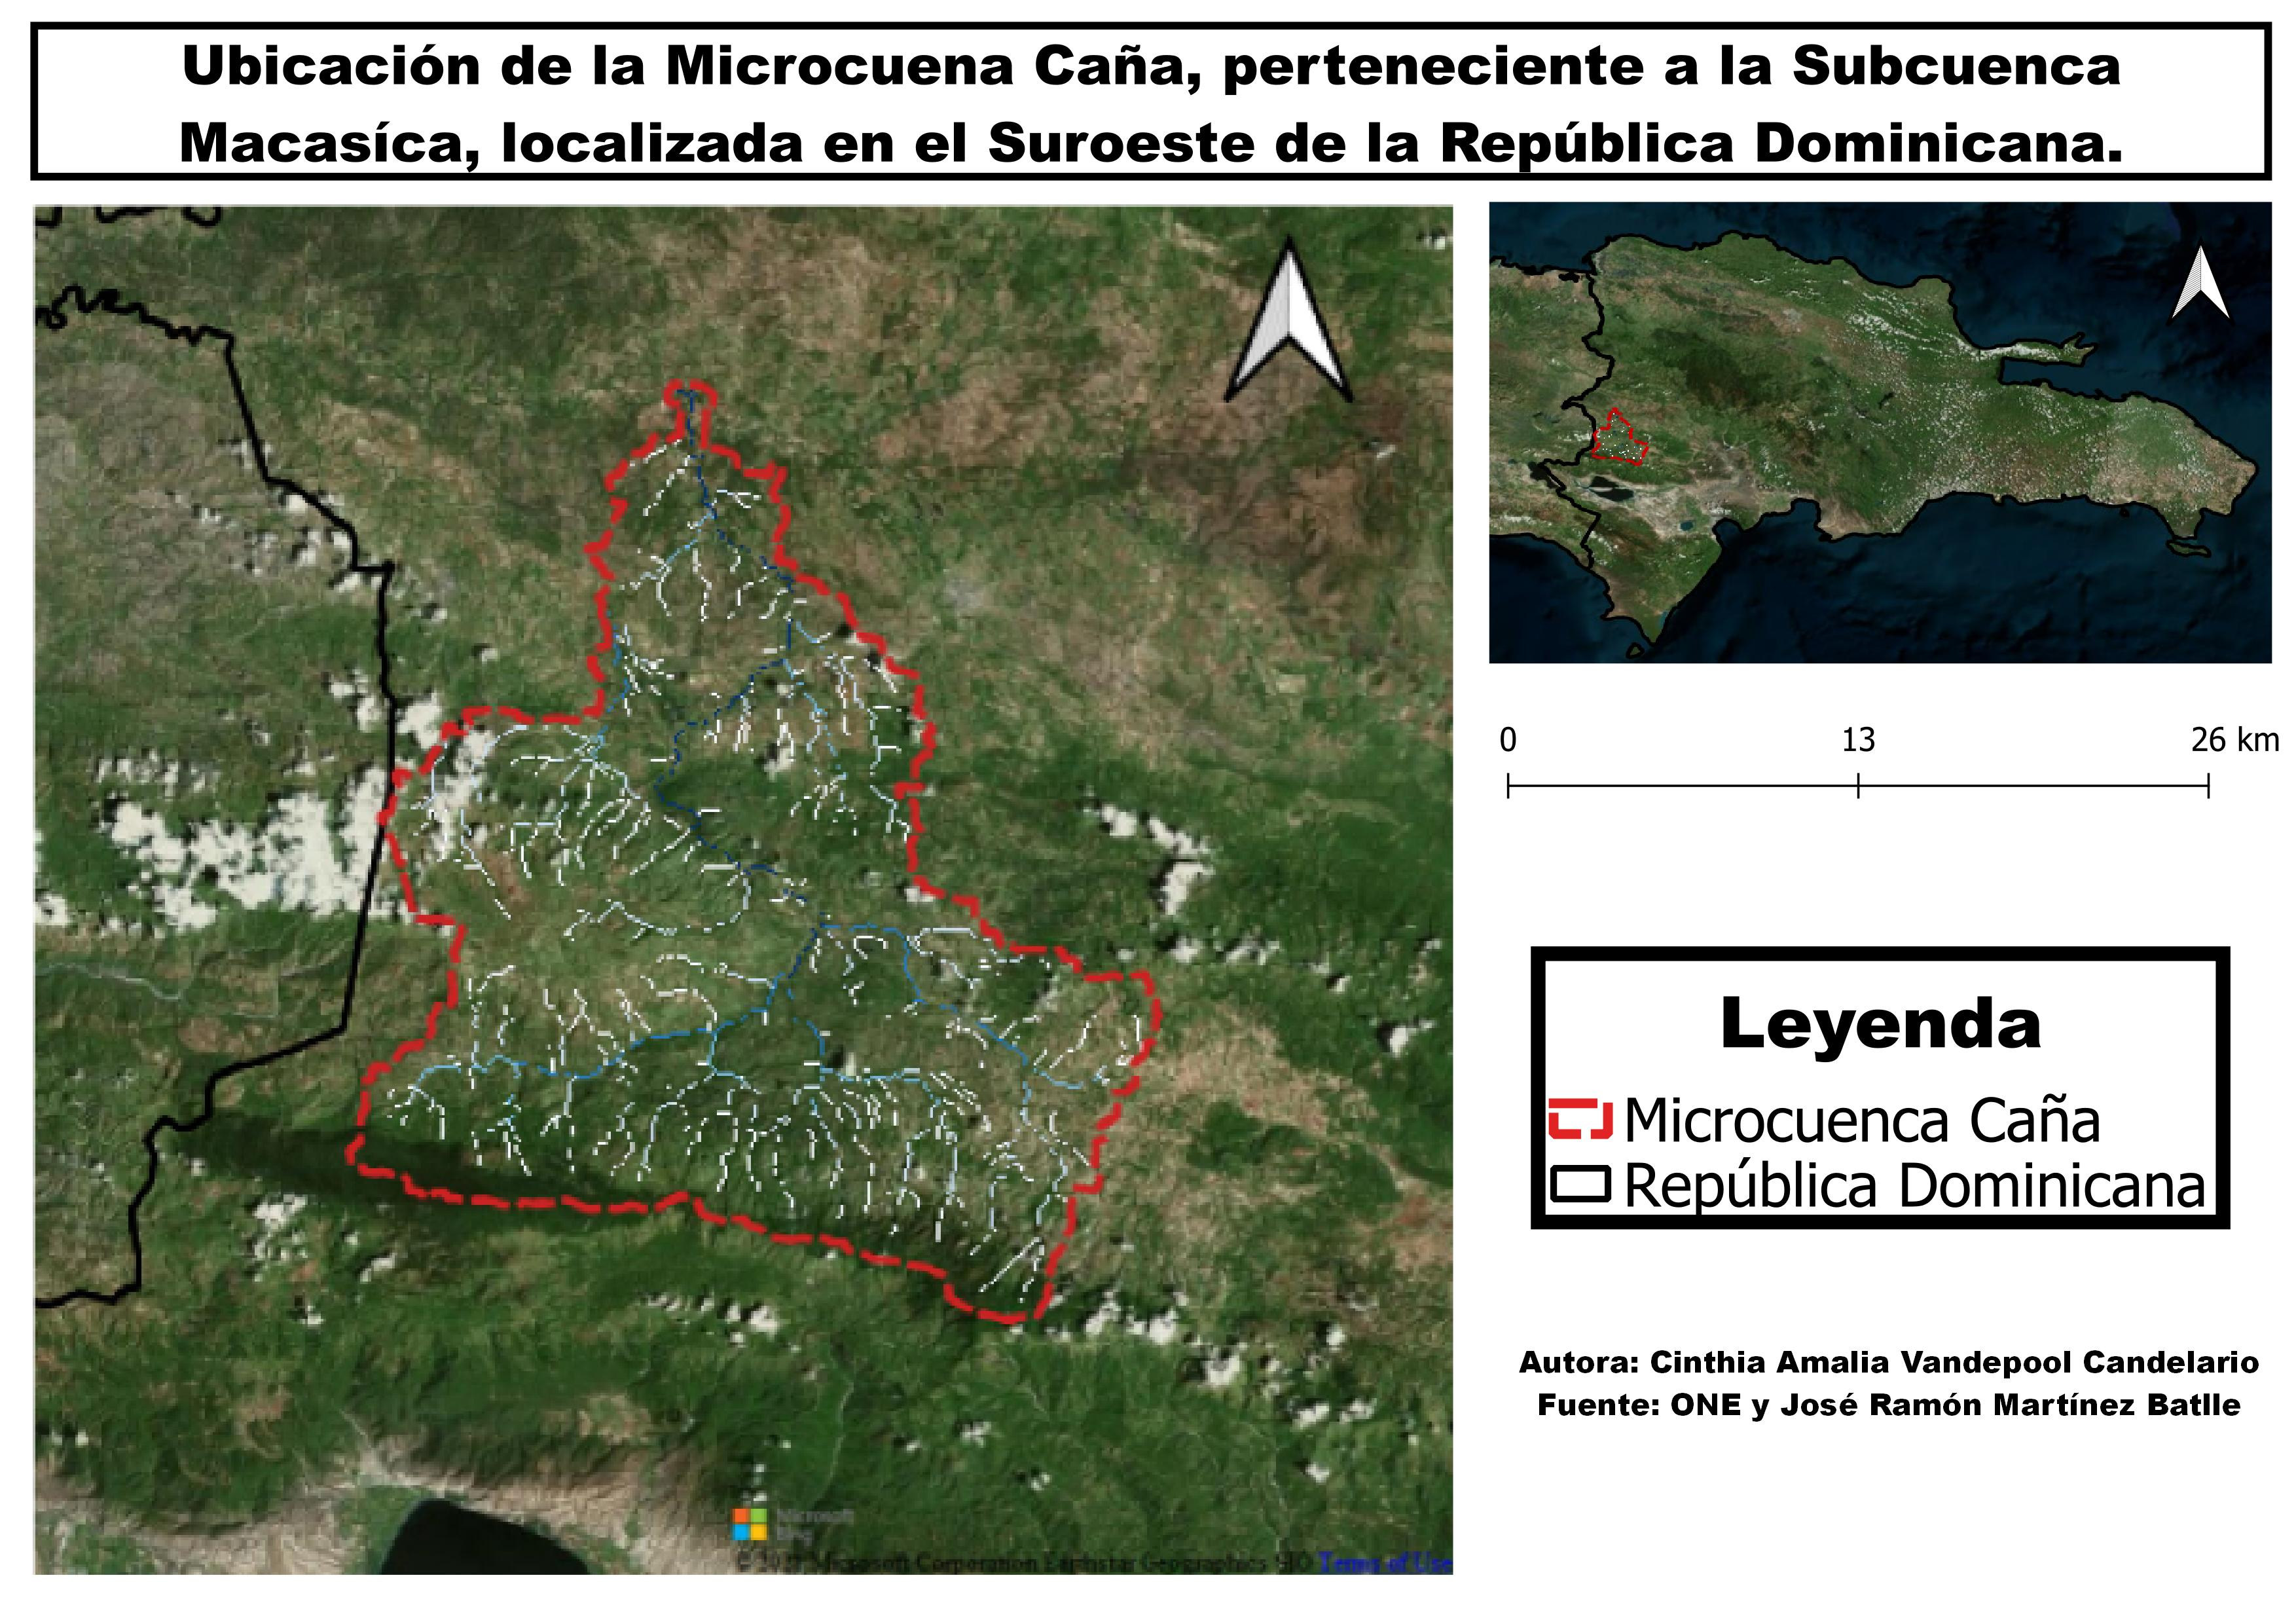
\includegraphics[width=0.75000\textwidth]{mapa_de_microcuenca_cana.jpg}
\caption{Ubicación Microcuenca del Rio Caña\label{mapacuenca}}
\end{figure}

De acuerdo al mapa Zonas de Vida (OEA, 1967), la mayor superficie de la
cuenca lo ocupa el Bosque húmedo subtropical, se caracteriza por
presentar topografía que varía desde plana hasta accidentada con un
patrón de lluvia que varía de 1000 mm. a 2000 mm. Según la ubicación de
las áreas, la biotemperatura media anual es de 23ºC a 24ºC con una
evapotranspiración potencial estimada en promedio de 20\% menor que la
precipitación media total anual. El Bosque muy húmedo Montano Bajo es la
segunda en extensión, se caracteriza por la presencia de escarchas
temporales, precipitaciones que alcanzar cantidades mayores a los 2,000
mm. totales anuales con una evapotranspiración potencial estimada en
promedio de 55\% menor que la precipitación media total anual, su
topografía generalmente accidentada con elevaciones que van desde los
850 hasta los 2,100 metros y en menor proporción lo ocupa el bosque
húmedo montano bajo (Ministerio de Medio ambiente y Recursos naturales,
2016).

La mayor parte de la cuenca se localiza sobre la vertiente Norte del
sistema geomorfológico de la Sierra de Neiba y, en menor proporción,
sobre el Valle de San juan, siendo la geología conformada, en mayor
proporción, por caliza tipo Neiba, marga con calcarenita tipo
sombrerito, marga con intercalaciones de bancos de caliza arenosa,
arenisca, marga arenosa, conglomerados, conglomerados poligénico, molasa
marina y continental y arena; y en menor proporción está conformada por
caliza en bancos de espesores variables con nódulos e intercalaciones de
pedernal de color blanco-crema, depósitos fluviales, depósitos
cuaternarios indiferenciados, basaltos, tobas, aglomerados y rocas
volcánicas submarinas (Ministerio de Medio ambiente y Recursos
naturales, 2016) (Ver figura \ref{mapageologico})

\begin{figure}
\centering
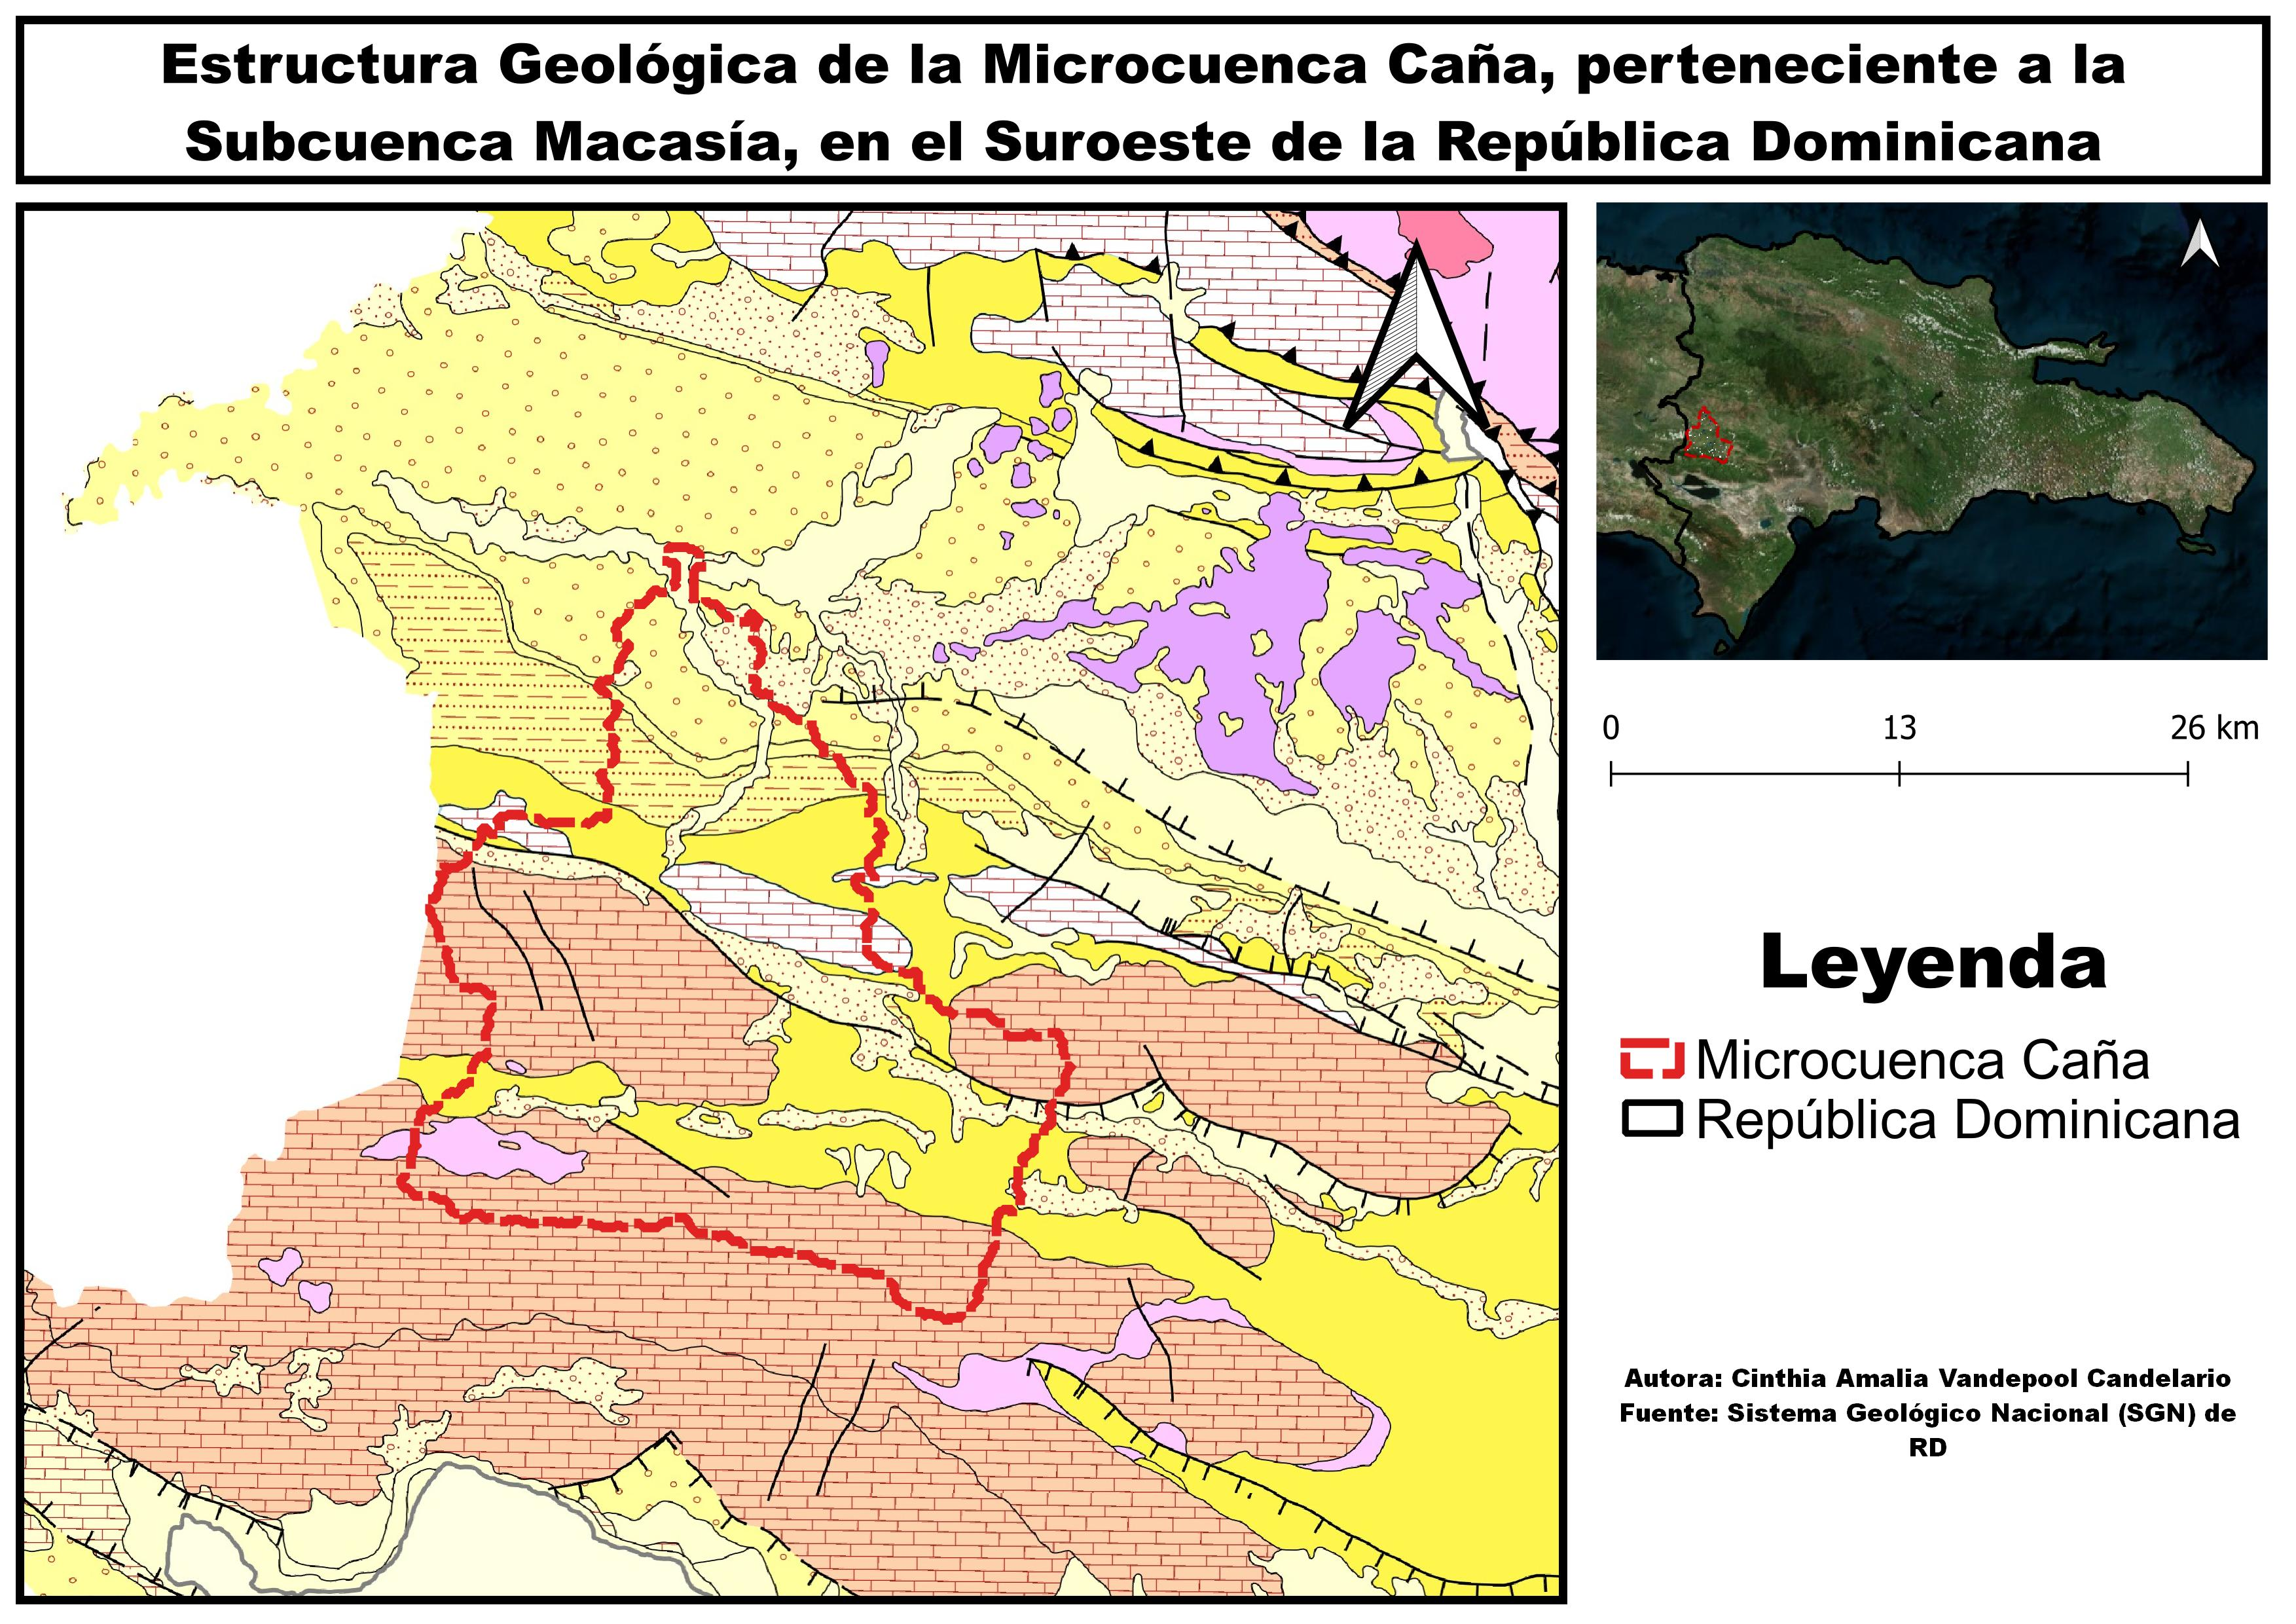
\includegraphics[width=0.75000\textwidth]{mapa_geologico_cuenca_cana.jpg}
\caption{Estructura Geológica de la Microcuenca
Caña\label{mapageologico}}
\end{figure}

\subsection{Materiales, fuentes de datos y
métodos}\label{materiales-fuentes-de-datos-y-muxe9todos}

Para la elaboración de esta investigación se emplearon métodos de
análisis morfométrico a partir de un modelo digital de elevación (MDE)
de la cuenca de interés, el cual es un modelo simbólico, de estructura
numérica y digital que pretende representar la distribución espacial de
la elevación del terreno, siendo la altura una variable escalar que se
distribuye en un espacio bidimensional (Burgos \& Salcedo, 2014);
inicialmente se cargó una serie de paquetes de R, con el objetivo de
adecuar el entorno para la ejecución de los códigos necesarios, entre
los que se destacan rgrass7, mapview, leaflet, tidyverse, entre otros
{[}@,{]}. El paquete rgrass7 se situó encima del software GRASS GIS
(GRASS Development Team, 1998--2021), siendo este último el que se
ejecutó en el \emph{backend} los algoritmos requeridos para producir los
resultados morfométricos, a continuación se detallaran los
procedimientos implementados.

En primer lugar, se importó a R, como SpatialGridDataFrame, un MDE
(Burgos \& Salcedo, 2014) alojado en la base de datos de GRASS GIS
(GRASS Development Team, 1998--2021), se estableció su ruta y
convirtiéndolo a su vez en un objeto raster por medio del paquete raster
de R; partiendo del complemento \emph{r.watershed} (el cual genera un
conjunto de mapas que indican: \emph{la acumulación de flujo, la
dirección del drenaje, la ubicación de los arroyos y las cuencas
hidrográficas} (GRASS Development Team, 2003g)) y del MDE se generaron
diversas capas calculando así los parámetros hidrográficos de la cuenca
del río caña y sus redes de drenaje, además, seguido a esto se importó
un conjunto de capas ráster de GRASS GIS a R, como el mapa de red de
drenaje y el mapa de cuencas visualizándolas por medio de
\emph{leaflet}.

Utilizando el complemento de GRASS GIS \emph{r.water.outlet} (GRASS
Development Team, 2003f) y apoyándose en los paquetes \emph{mapview}
(Tim Appelhans and others, 2020) y \emph{leaflet} se extrajo la cuenca
de drenaje a partir de un mapa de dirección de flujos con un umbral de
acumulación de \emph{80 celdas} y las coordenadas de la desembocadura de
la cuenca cana (-71.62524,18.94026).

Posteriormente se estableció una máscara usando el límite de la cuenca
Caña para luego realizar la extracción partir del MDE de la red de
drenaje utilizando el complemento de GRASS GIS \emph{r.stream.extract}
(GRASS Development Team, 2003d) desde R. Tras esto, se utilizó el
complemento \emph{r.stream}(GRASS Development Team, 2003e) para generar
un mapa de dirección de flujo, \emph{r.stream.order} (GRASS Development
Team, 2003b) para un mapa de orden de red según varios métodos, entre
ellos el método de Strahler y de Horton, a partir de
\emph{r.stream.basins} (GRASS Development Team, 2003c) un mapa de
cuencas según órdenes de red y apoyándose del complemento
\emph{r.stream.stats}(GRASS Development Team, 2003a) se generó las
estadísticas de red resumidas por órdenes, incluyendo la razón de
bifurcación.

Por último, obtuvimos el curso más largo de la microcuenca a partir de
la función \emph{LfpNetwork} creada por José Ramón Martínez (Batlle,
2021), con la misma función, además, pudimos obtener los cursos más
largos de las cuencas tributarias. Seguido a esto se generaron los
perfiles longitudinales de la microcuenca, se calcularon sus índices de
concavidad y a partir de las herramientas \emph{QGIS} y \emph{Google
EARTH} cruzamos la información geológica con los patrones de
concavidad/convexidad.

\section{Resultados}\label{resultados}

A partir de los códigos ejecutados determinamos que la microcuenca del
río caña posee una superficie de 525 km\textsuperscript{2} con un
perímetro de 139 km, presentando una forma similar a la de un triángulo,
presenta mayor extensión en el Sur reduciendo su extensión así el Norte.
(figura \ref{areacuenca}). Esta microcuenca posee una elevación máxima
de 2,231 metros sobre el nivel del mar, una elevación mínima de 330
metros sobre el nivel del mar y una elevación media de 958 metros.
Además, presenta una pendiente media de 10.56 (figura\ref{pendiente}
figura \ref{mapadependiente}).

\begin{figure}
\centering
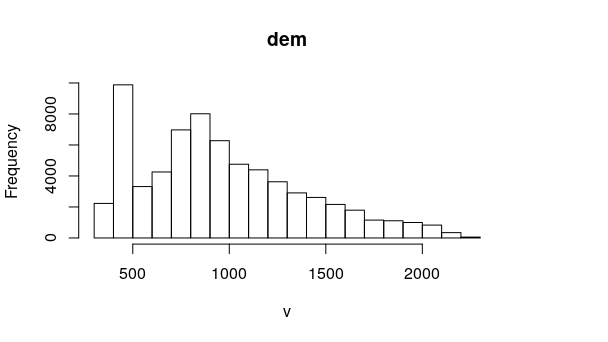
\includegraphics[width=0.50000\textwidth]{pendiente_cana.png}
\caption{Pendiente\label{pendiente}}
\end{figure}

La red de drenaje de la microcuenca Caña posee longitud de 445
km\textsuperscript{2} distribuidos en 271 cursos de fluviales con una
densidad de drenaje de 0.82 km/km\textsuperscript{2}, además el orden
máximo alcanzado fue de 5.(figura \ref{reddrenaje}) (Ver
tabla\ref{tab:cursosfluviales}). La mayor parte de la red discurre por
caliza, marga y conglomerados; En el tramo alto de la cuenca la red de
drenaje es más ancha, concentrándose en esta zona la mayor parte de los
cursos mientras en la zona intermedia la red se encoge, disminuyendo
también el número de cursos fluviales.

Esta red presenta un patrón de drenaje mixto siendo predominantemente un
patrón detrítico en la cuenca media, rectangular en parte alta y baja y
paralelo en algunas zonas de la cuenca media. En la zona en donde se
presenta un patrón detrítico coincide con calizas, margas y basalto, en
la zona en donde predomina el patrón de drenaje rectangular se
encuentran rocas de tipo caliza de la formación Neiba y conglomerados
mientras en la zona que se encuentra un patrón paralelo predominan las
margas y las areniscas.

\begin{figure}
\centering
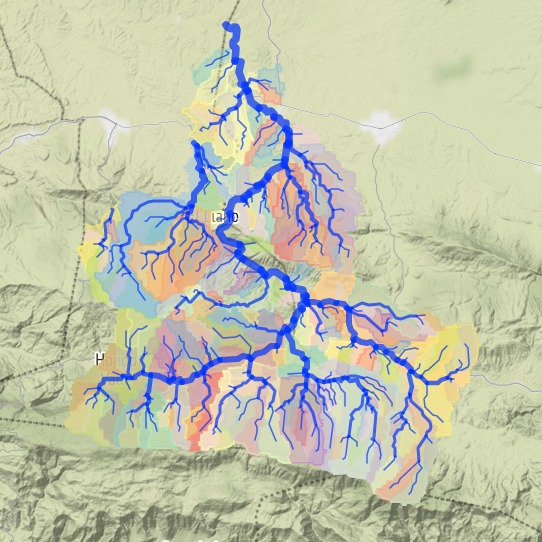
\includegraphics[width=0.57000\textwidth]{mapa_orden_de_red.jpeg}
\caption{Red de drenaje de la microcuenca Caña\label{reddrenaje}}
\end{figure}

\begin{longtable}[]{@{}cc@{}}
\caption{\label{tab:cursosfluviales} Número de Cursos fluviales en
función del Orden}\tabularnewline
\toprule
Orden de Red & No. de Cursos fluviales\tabularnewline
\midrule
\endfirsthead
\toprule
Orden de Red & No. de Cursos fluviales\tabularnewline
\midrule
\endhead
1 & 204\tabularnewline
2 & 50\tabularnewline
3 & 12\tabularnewline
4 & 4\tabularnewline
5 & 1\tabularnewline
\bottomrule
\end{longtable}

A continuación, se indicarán la razón de bifurcación de todos los
órdenes de red de la microcuenca caña, utilizando dos procedimientos
distintos: La razón de bifurcación promedio del par de órdenes
1\textbar{}2 es 204/50=4.08, para el par de órdenes 2\textbar{}3 es
50/12=4.16, para el par de órdenes 3\textbar{}4 es 12/4=3 y para el par
de órdenes 4\textbar{}5 es 4/1=4; el valor promedio es Rb= 3.811667.
Mientras que la razón de bifurcación por medio de coeficientes de
regresión es Rb= 3.7292 (figura\ref{razonbifurcacion}). Además, pudimos
observar que las ramificaciones de orden 1 y 2 son las que presentan un
grado de bifurcación más alto, las cuales discurren, en mayor
proporción, sobre caliza de tipo Neiba y Marga.

\begin{figure}
\centering
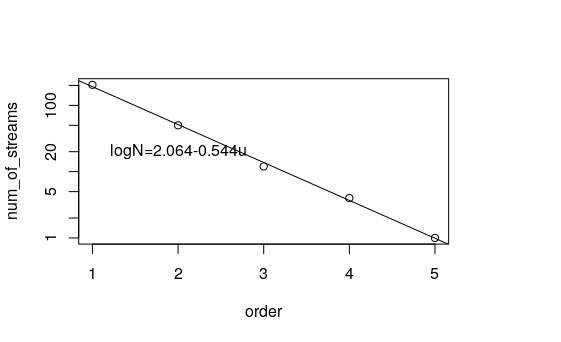
\includegraphics{razon_de_bifurcacion.png}
\caption{Recta de regresión para el modelo ``número de cursos fluviales
es función del orden de red'' y ecuación
correspondiente\label{razonbifurcacion}}
\end{figure}

EL curso más largo posee una longitud de 58.1 Kilómetros y discurre por
el lado occidental de la cuenca, sobre una falla que atravieza la cuenca
en su zona intermedia (figura \ref{cursolargo}). En función de los
resultados obtenidos, se observó que la mayor parte de los cursos
fluviales de la microcuenca presentan un perfil cóncavo y en pocas
ocasiones presentan un perfil convexo, provocado esto por estar en zona
de cabecera o por discurrir sobre depósitos aluviales; además, algunos
flujos presentan un perfil rectilíneo que también puede deberse al tipo
de material por el que discurre.

\begin{figure}
\centering
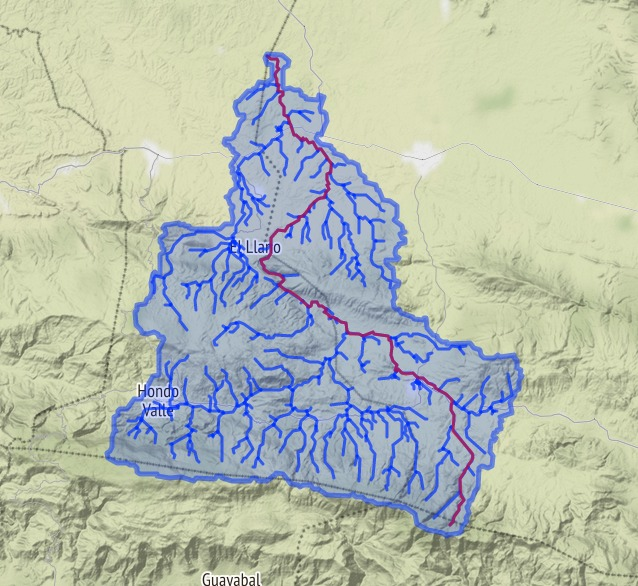
\includegraphics{curso_mas_largo.jpeg}
\caption{Curso fluvial más largo de la Microcuenca
Caña\label{cursolargo}}
\end{figure}

\begin{figure}
\centering
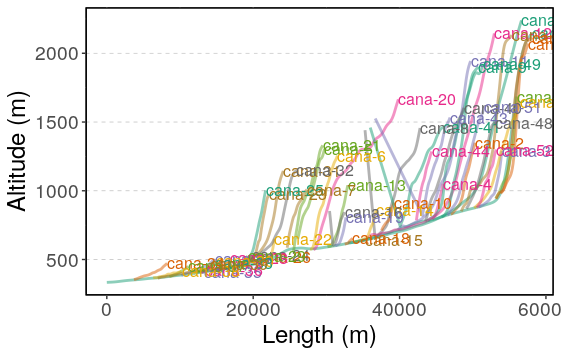
\includegraphics{perfiles_cana.png}
\caption{Perfil de Concavidad\label{perfilconcavidad}}
\end{figure}

\begin{figure}
\centering
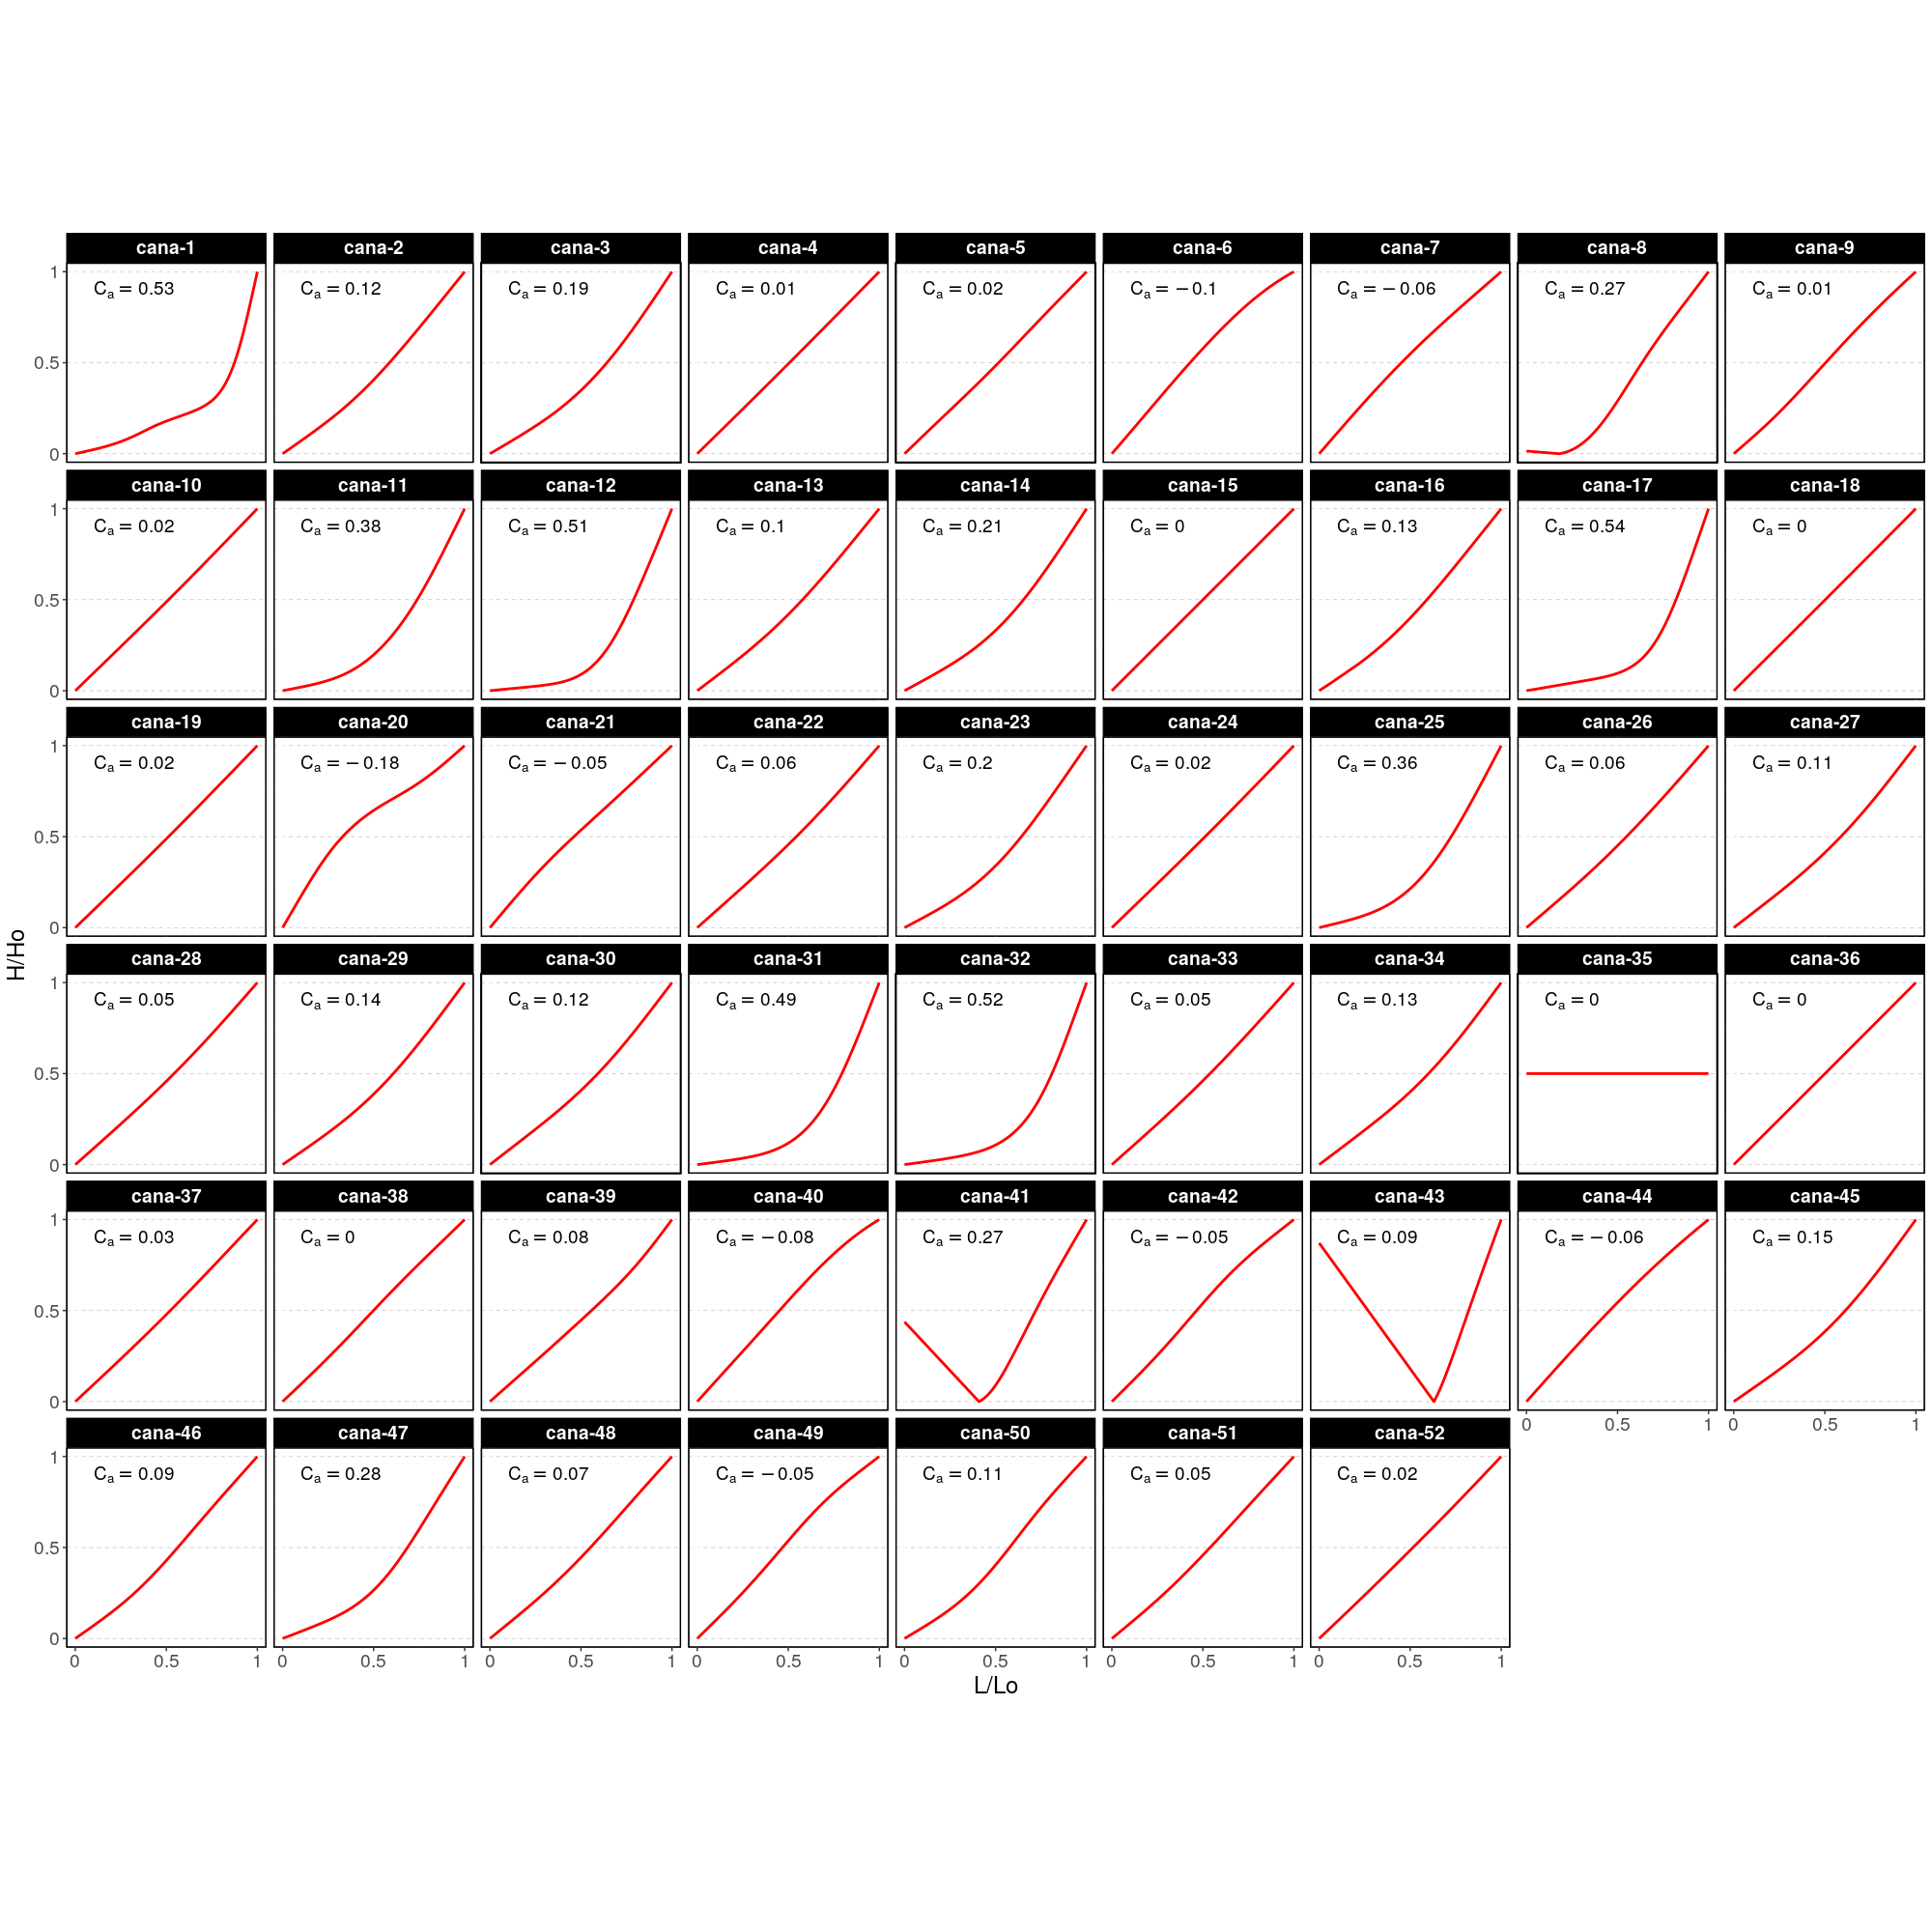
\includegraphics{indice_concavidad.png}
\caption{Indice de Concavidad\label{indiceconcavidad}}
\end{figure}

A continuacion se resumen algunos parametros morfométricos no
mencionados anteriormente: (Ver tabla\ref{tab:parametrosmorfo})

\begin{longtable}[]{@{}cc@{}}
\caption{\label{tab:parametrosmorfo} Parametros Morfometricos de la
Microcuenca Caña}\tabularnewline
\toprule
\begin{minipage}[b]{0.75\columnwidth}\centering\strut
Parámetros\strut
\end{minipage} & \begin{minipage}[b]{0.19\columnwidth}\centering\strut
Valores\strut
\end{minipage}\tabularnewline
\midrule
\endfirsthead
\toprule
\begin{minipage}[b]{0.75\columnwidth}\centering\strut
Parámetros\strut
\end{minipage} & \begin{minipage}[b]{0.19\columnwidth}\centering\strut
Valores\strut
\end{minipage}\tabularnewline
\midrule
\endhead
\begin{minipage}[t]{0.75\columnwidth}\centering\strut
Orientación Centroide de la cuenca\strut
\end{minipage} & \begin{minipage}[t]{0.19\columnwidth}\centering\strut
226125.00\strut
\end{minipage}\tabularnewline
\begin{minipage}[t]{0.75\columnwidth}\centering\strut
Norte Centroide de la cuenca\strut
\end{minipage} & \begin{minipage}[t]{0.19\columnwidth}\centering\strut
2075805.00\strut
\end{minipage}\tabularnewline
\begin{minipage}[t]{0.75\columnwidth}\centering\strut
Rectángulo que contiene la cuenca N-O\strut
\end{minipage} & \begin{minipage}[t]{0.19\columnwidth}\centering\strut
(`211500', `2096370')\strut
\end{minipage}\tabularnewline
\begin{minipage}[t]{0.75\columnwidth}\centering\strut
Rectángulo que contiene la cuenca S-E\strut
\end{minipage} & \begin{minipage}[t]{0.19\columnwidth}\centering\strut
(`241650', `2061540')\strut
\end{minipage}\tabularnewline
\begin{minipage}[t]{0.75\columnwidth}\centering\strut
Longitud del vector director {[}km{]}\strut
\end{minipage} & \begin{minipage}[t]{0.19\columnwidth}\centering\strut
20.63435024419233\strut
\end{minipage}\tabularnewline
\begin{minipage}[t]{0.75\columnwidth}\centering\strut
Orientación predominante {[}grado desde el norte, en sentido contrario a
las agujas del reloj{]}\strut
\end{minipage} & \begin{minipage}[t]{0.19\columnwidth}\centering\strut
1.4441150421051312\strut
\end{minipage}\tabularnewline
\begin{minipage}[t]{0.75\columnwidth}\centering\strut
Coeficiente de compacidad\strut
\end{minipage} & \begin{minipage}[t]{0.19\columnwidth}\centering\strut
5.390348659271303\strut
\end{minipage}\tabularnewline
\begin{minipage}[t]{0.75\columnwidth}\centering\strut
Relación de circularidad\strut
\end{minipage} & \begin{minipage}[t]{0.19\columnwidth}\centering\strut
0.33967691382621185\strut
\end{minipage}\tabularnewline
\begin{minipage}[t]{0.75\columnwidth}\centering\strut
Diámetro topológico\strut
\end{minipage} & \begin{minipage}[t]{0.19\columnwidth}\centering\strut
53.0\strut
\end{minipage}\tabularnewline
\begin{minipage}[t]{0.75\columnwidth}\centering\strut
Relación de alargamiento\strut
\end{minipage} & \begin{minipage}[t]{0.19\columnwidth}\centering\strut
0.472103656324998\strut
\end{minipage}\tabularnewline
\begin{minipage}[t]{0.75\columnwidth}\centering\strut
Factor de forma\strut
\end{minipage} & \begin{minipage}[t]{0.19\columnwidth}\centering\strut
9.58527016453617\strut
\end{minipage}\tabularnewline
\begin{minipage}[t]{0.75\columnwidth}\centering\strut
Tiempo de concentración (Giandotti, 1934) {[}hr{]}\strut
\end{minipage} & \begin{minipage}[t]{0.19\columnwidth}\centering\strut
4.981885705233938\strut
\end{minipage}\tabularnewline
\begin{minipage}[t]{0.75\columnwidth}\centering\strut
Longitud del canal principal {[}km{]}\strut
\end{minipage} & \begin{minipage}[t]{0.19\columnwidth}\centering\strut
54.757012947\strut
\end{minipage}\tabularnewline
\begin{minipage}[t]{0.75\columnwidth}\centering\strut
Pendiente media del canal principal {[}porcentaje{]}\strut
\end{minipage} & \begin{minipage}[t]{0.19\columnwidth}\centering\strut
3.57379418847005\strut
\end{minipage}\tabularnewline
\begin{minipage}[t]{0.75\columnwidth}\centering\strut
Longitud media de la ladera {[}m{]}\strut
\end{minipage} & \begin{minipage}[t]{0.19\columnwidth}\centering\strut
152.0461\strut
\end{minipage}\tabularnewline
\begin{minipage}[t]{0.75\columnwidth}\centering\strut
Magnitud\strut
\end{minipage} & \begin{minipage}[t]{0.19\columnwidth}\centering\strut
147.0\strut
\end{minipage}\tabularnewline
\begin{minipage}[t]{0.75\columnwidth}\centering\strut
Frecuencia de flujo de primer orden\strut
\end{minipage} & \begin{minipage}[t]{0.19\columnwidth}\centering\strut
0.2800742797000376\strut
\end{minipage}\tabularnewline
\begin{minipage}[t]{0.75\columnwidth}\centering\strut
Relación de longitud (Horton)\strut
\end{minipage} & \begin{minipage}[t]{0.19\columnwidth}\centering\strut
2.1685\strut
\end{minipage}\tabularnewline
\begin{minipage}[t]{0.75\columnwidth}\centering\strut
Ratio de superficie (Horton)\strut
\end{minipage} & \begin{minipage}[t]{0.19\columnwidth}\centering\strut
3.9485\strut
\end{minipage}\tabularnewline
\begin{minipage}[t]{0.75\columnwidth}\centering\strut
Relación de inclinación (Horton)\strut
\end{minipage} & \begin{minipage}[t]{0.19\columnwidth}\centering\strut
1.6639\strut
\end{minipage}\tabularnewline
\bottomrule
\end{longtable}

\section{Discusión}\label{discusiuxf3n}

Gracias a las investigaciones y observaciones realizadas se obtuvieron
las características morfométricas de la microcuenca Caña. Concretamente
se determinó que esta microcuenca presenta un patrón de drenaje
detrítico, rectangular y paralelo que según (Elorza, 2008) se debe a la
interacción entre el flujo y los materiales erosionables y también se
observó que la densidad de drenaje de la microcuenca es baja (0.82
km/km\textsuperscript{2}) lo que se interpreta en que los suelos de la
cuenca son poco erosionables y presentan escasa capa vegetal (Manuel
Córdova, 2016).

También, al superponer la red de drenaje sobre el mapa geológico
nacional, se observó que existen la posibilidad de un proceso de
reorganizamiento del drenaje, ya que la mayor parte de este curso
discurre sobre rocas calizas y margas, de la misma forma se observó que
la cuenca es atravesada en su parte intermedia por una falla, que puedo
provocar el encogimiento de la red en la parte media-baja. Además, por
medio del estudio de la red de drenaje, creemos que el curso principal
pudo haber atravesado por un proceso de migración lateral, proceso que
pudo ser producto del movimiento de tectónico.

Del mismo modo, se analizó el índice de concavidad de la microcuenca
observando que en su mayoría los cursos fluviales presentan un perfil
cóncavo, otra parte presentan un perfil convexo y una minoría un perfil
rectilíneo; el resultado de los índices cóncavos y convexos se pueden
deber a la zona por la que discurre esos cursos ya sea en zona de
cabecera o sobre depósitos aluviales, con relación al perfil rectilíneo
pocos autores hacen referencia de este por lo que será necesario llevar
a cabo nuevas investigaciones.

Con relación a la razón de bifurcación, según Horton (1945) esta razón
debe ser constante entre un par de órdenes y el otro, pero en la
microcuenca de estudio esto no sucede, aunque estas variaciones fueron
mínimas se requerirán estudios más profundos para determinar si esto es
producto de las variaciones climáticas o litológicas de esta zona,
observando, además, que el cálculo de la razón de bifurcación promedio y
la razón de bifurcación por medio de coeficientes de regresión obtuvimos
valores distintos, pero con una diferencia pequeña (0.08).

Como consecuencia de los hallazgos de esta investigación se calcularon
algunos de los parámetros morfométricos de la microcuenca Caña, sin
embargo, este trabajo solo representa la base para formular nuevas
hipótesis que requerirán nuevas investigaciones, no solo de esta
microcuenca sino también en todos los sistemas fluviales de la isla, ya
que este tipo de estudios son escasos o inexistentes en nuestro país.

\section{Agradecimientos}\label{agradecimientos}

\section{Información de soporte}\label{informaciuxf3n-de-soporte}

\ldots

\section{\texorpdfstring{\emph{Script}
reproducible}{Script reproducible}}\label{script-reproducible}

\begin{Shaded}
\begin{Highlighting}[]
\CommentTok{#parte reutizable del script ----}
\CommentTok{#cargar paquetes}
\KeywordTok{library}\NormalTok{(rgrass7)}
\KeywordTok{library}\NormalTok{(sp)}
\KeywordTok{library}\NormalTok{(sf)}
\KeywordTok{library}\NormalTok{(raster)}
\NormalTok{gisdbase <-}\StringTok{ 'grass-data-test'} \CommentTok{#Base de datos de GRASS GIS}
\NormalTok{wd <-}\StringTok{ }\KeywordTok{getwd}\NormalTok{() }\CommentTok{#Directorio de trabajo}
\NormalTok{wd}
\NormalTok{loc <-}\StringTok{ }\KeywordTok{initGRASS}\NormalTok{(}\DataTypeTok{gisBase =} \StringTok{"/usr/lib/grass78/"}\NormalTok{,}
                 \DataTypeTok{home =}\NormalTok{ wd,}
                 \DataTypeTok{gisDbase =} \KeywordTok{paste}\NormalTok{(wd, gisdbase, }\DataTypeTok{sep =} \StringTok{'/'}\NormalTok{),}
                 \DataTypeTok{location =} \StringTok{'cana'}\NormalTok{,}
                 \DataTypeTok{mapset =} \StringTok{"PERMANENT"}\NormalTok{,}
                 \DataTypeTok{override =} \OtherTok{TRUE}\NormalTok{)}

\CommentTok{#unlink_.gislock()}

\CommentTok{#Fin de la parte reutilizable}

\CommentTok{#video 4 ----}
\CommentTok{#Definir proyección de la región de GRASS GIS, importar fuente y utilizarla para definir extensión y resolución. Cómo ver la ayuda de las funciones}
\CommentTok{#Muestra la definición de la región}
\KeywordTok{gmeta}\NormalTok{()}
\CommentTok{#Definir ruta del DEM}
\NormalTok{dem <-}\StringTok{ 'datos-fuente/srtm_dem_cuenca_cana.tif'}

\CommentTok{#Definir la proyección de la región basada en DEM}
\KeywordTok{execGRASS}\NormalTok{(}
  \DataTypeTok{cmd =} \StringTok{'g.proj'}\NormalTok{,}
  \DataTypeTok{flags =} \KeywordTok{c}\NormalTok{(}\StringTok{'t'}\NormalTok{,}\StringTok{'c'}\NormalTok{),}
  \DataTypeTok{georef=}\NormalTok{dem)}
\CommentTok{#Muestra la definición de la región modificada}
\KeywordTok{gmeta}\NormalTok{()}

\CommentTok{#Importar mapa raster}
\CommentTok{#r.in.gdal importa la fuente a GRASS}
\KeywordTok{execGRASS}\NormalTok{(}
  \DataTypeTok{cmd =} \StringTok{'r.in.gdal'}\NormalTok{,}
  \DataTypeTok{flags=}\KeywordTok{c}\NormalTok{(}\StringTok{'overwrite'}\NormalTok{,}\StringTok{'quiet'}\NormalTok{),}
  \DataTypeTok{parameters=}\KeywordTok{list}\NormalTok{(}
    \DataTypeTok{input=}\NormalTok{dem,}
    \DataTypeTok{output=}\StringTok{'dem'}
\NormalTok{  )}
\NormalTok{)}
\CommentTok{#Actualizar la extensión de la región al DEM, sólo por precaución}
\KeywordTok{execGRASS}\NormalTok{(}
  \DataTypeTok{cmd =} \StringTok{'g.region'}\NormalTok{,}
  \DataTypeTok{parameters=}\KeywordTok{list}\NormalTok{(}
    \DataTypeTok{raster =} \StringTok{'dem'}\NormalTok{,}
    \DataTypeTok{align =} \StringTok{'dem'}
\NormalTok{  )}
\NormalTok{)}
\CommentTok{#Importar un mapa vectorial también}
\NormalTok{demext <-}\StringTok{ 'datos-fuente/cuenca_cana.geojson'}
\KeywordTok{execGRASS}\NormalTok{(}
  \DataTypeTok{cmd =} \StringTok{'v.in.ogr'}\NormalTok{,}
  \DataTypeTok{flags=}\KeywordTok{c}\NormalTok{(}\StringTok{'overwrite'}\NormalTok{,}\StringTok{'quiet'}\NormalTok{),}
  \DataTypeTok{parameters=}\KeywordTok{list}\NormalTok{(}
    \DataTypeTok{input=}\NormalTok{demext,}
    \DataTypeTok{output=}\StringTok{'dem_extent'}
\NormalTok{  )}
\NormalTok{)}
\CommentTok{#Imprimir lista de mapas ráster y vectoriales dentro en la región/localización activa}
\KeywordTok{execGRASS}\NormalTok{(}
  \StringTok{'g.list'}\NormalTok{,}
  \DataTypeTok{flags =} \StringTok{'t'}\NormalTok{,}
  \DataTypeTok{parameters =} \KeywordTok{list}\NormalTok{(}
    \DataTypeTok{type =} \KeywordTok{c}\NormalTok{(}\StringTok{'raster'}\NormalTok{, }\StringTok{'vector'}\NormalTok{)}
\NormalTok{  )}
\NormalTok{)}
\CommentTok{#Ver los addons disponibles en el repositorio oficial de GRASS GIS, incluyendo descripción}
\KeywordTok{execGRASS}\NormalTok{(}
  \DataTypeTok{cmd =} \StringTok{'g.extension'}\NormalTok{,}
  \DataTypeTok{flags =} \StringTok{'c'}
\NormalTok{)}

\CommentTok{#Video 5 Explorar datos espaciales básicos entre GRASS y R ----}
\CommentTok{#Cargar en R el DEM (mapa ráster)}
\KeywordTok{use_sp}\NormalTok{()}
\NormalTok{dem_sp <-}\StringTok{ }\KeywordTok{readRAST}\NormalTok{(}\StringTok{'dem'}\NormalTok{)}
\NormalTok{op <-}\StringTok{ }\KeywordTok{par}\NormalTok{()}
\KeywordTok{plot}\NormalTok{(dem_sp)}

\CommentTok{#Cargar a R el mapa vectorial de una cuenca que se encuentra alojado fuera de GRASS, hacer el plot y representar la cuenca del rio cana superpuesta}
\NormalTok{rutacana <-}\StringTok{ 'datos-fuente/cuenca_cana.geojson'}
\NormalTok{cana <-}\StringTok{ }\KeywordTok{st_read}\NormalTok{(rutacana)}
\KeywordTok{plot}\NormalTok{(dem_sp)}
\KeywordTok{plot}\NormalTok{(cana, }\DataTypeTok{add=}\NormalTok{T, }\DataTypeTok{col=}\StringTok{'transparent'}\NormalTok{, }\DataTypeTok{border=}\StringTok{'black'}\NormalTok{, }\DataTypeTok{lwd=}\DecValTok{5}\NormalTok{);}\KeywordTok{par}\NormalTok{(op[}\KeywordTok{c}\NormalTok{(}\StringTok{'mfrow'}\NormalTok{,}\StringTok{'mar'}\NormalTok{)])}

\CommentTok{#Analizar el DEM dentro de la cuenca del rio cana}
\NormalTok{dem_r0 <-}\StringTok{ }\KeywordTok{raster}\NormalTok{(dem_sp)}
\NormalTok{dem_r1 <-}\StringTok{ }\KeywordTok{crop}\NormalTok{(dem_r0, cana)}
\NormalTok{dem_cana <-}\StringTok{ }\KeywordTok{mask}\NormalTok{(dem_r1, cana)}
\KeywordTok{plot}\NormalTok{(dem_cana)}

\KeywordTok{summary}\NormalTok{(dem_cana)}
\KeywordTok{hist}\NormalTok{(dem_cana)}

\CommentTok{#Obtener variables de terreno básicas con el paquete raster dentro de R}
\NormalTok{pend_cana <-}\StringTok{ }\KeywordTok{terrain}\NormalTok{(}\DataTypeTok{x =}\NormalTok{ dem_cana, }\DataTypeTok{opt =} \StringTok{'slope'}\NormalTok{, }\DataTypeTok{unit =} \StringTok{'degrees'}\NormalTok{)}
\KeywordTok{plot}\NormalTok{(pend_cana)}
\end{Highlighting}
\end{Shaded}

\begin{Shaded}
\begin{Highlighting}[]
\CommentTok{#video 6 Calcular parámetros hidrográficos con r.watershed. Visualizar con leaflet ----}
\CommentTok{# Calcular parámetros hidrográficos de interés usando `r.watershed`}
\KeywordTok{execGRASS}\NormalTok{(}
  \StringTok{"r.watershed"}\NormalTok{,}
  \DataTypeTok{flags =} \KeywordTok{c}\NormalTok{(}\StringTok{'overwrite'}\NormalTok{,}\StringTok{'quiet'}\NormalTok{),}
  \DataTypeTok{parameters =} \KeywordTok{list}\NormalTok{(}
    \DataTypeTok{elevation =} \StringTok{"dem"}\NormalTok{,}
    \DataTypeTok{accumulation =} \StringTok{"accum-de-rwshed"}\NormalTok{,}
    \DataTypeTok{stream =} \StringTok{"stream-de-rwshed"}\NormalTok{,}
    \DataTypeTok{drainage =} \StringTok{"drainage-dir-de-rwshed"}\NormalTok{,}
    \DataTypeTok{basin =} \StringTok{'basins'}\NormalTok{,}
    \DataTypeTok{half_basin =} \StringTok{'half-basins'}\NormalTok{,}
    \DataTypeTok{threshold =} \DecValTok{80}
\NormalTok{  )}
\NormalTok{)}
\CommentTok{# Traer capas a R}
\CommentTok{#Usar Spatial*}
\KeywordTok{library}\NormalTok{(sp)}
\KeywordTok{use_sp}\NormalTok{()}
\CommentTok{#Paquete manejo de los raster}
\KeywordTok{library}\NormalTok{(raster)}
\CommentTok{#DEM}
\NormalTok{dem <-}\StringTok{ }\KeywordTok{raster}\NormalTok{(}\KeywordTok{readRAST}\NormalTok{(}\StringTok{'dem'}\NormalTok{))}
\CommentTok{#Basins}
\NormalTok{basins <-}\StringTok{ }\KeywordTok{raster}\NormalTok{(}\KeywordTok{readRAST}\NormalTok{(}\StringTok{'basins'}\NormalTok{))}
\CommentTok{#Stream network}
\NormalTok{stream <-}\StringTok{ }\KeywordTok{raster}\NormalTok{(}\KeywordTok{readRAST}\NormalTok{(}\StringTok{'stream-de-rwshed'}\NormalTok{))}
\NormalTok{stream3857 <-}\StringTok{ }\KeywordTok{projectRaster}\NormalTok{(stream, }\DataTypeTok{crs =} \KeywordTok{CRS}\NormalTok{(}\StringTok{"+init=epsg:3857"}\NormalTok{), }\DataTypeTok{method =} \StringTok{'ngb'}\NormalTok{)}
\CommentTok{#Generar un vectorial de extensión de capa en EPSG:4326}
\NormalTok{e <-}\StringTok{ }\KeywordTok{extent}\NormalTok{(stream)}
\NormalTok{e <-}\StringTok{ }\KeywordTok{as}\NormalTok{(e, }\StringTok{'SpatialPolygons'}\NormalTok{)}
\KeywordTok{proj4string}\NormalTok{(e) <-}\StringTok{ }\KeywordTok{CRS}\NormalTok{(}\StringTok{"+init=epsg:32619"}\NormalTok{)}
\NormalTok{e <-}\StringTok{ }\KeywordTok{spTransform}\NormalTok{(e, }\DataTypeTok{CRSobj =} \KeywordTok{CRS}\NormalTok{(}\StringTok{"+init=epsg:4326"}\NormalTok{))}

\CommentTok{# Visualizar capas con `leaflet`}
\KeywordTok{library}\NormalTok{(leaflet)}
\KeywordTok{library}\NormalTok{(leafem)}
\KeywordTok{leaflet}\NormalTok{() }\OperatorTok
\StringTok{  }\KeywordTok{addProviderTiles}\NormalTok{(providers}\OperatorTok{$}\NormalTok{Stamen.Terrain, }\DataTypeTok{group =} \StringTok{'terrain'}\NormalTok{) }\OperatorTok
\StringTok{  }\KeywordTok{addRasterImage}\NormalTok{(dem, }\DataTypeTok{group=}\StringTok{'DEM'}\NormalTok{, }\DataTypeTok{opacity =} \FloatTok{0.5}\NormalTok{) }\OperatorTok
\StringTok{  }\KeywordTok{addRasterImage}\NormalTok{(}
    \KeywordTok{ratify}\NormalTok{(basins),}
    \DataTypeTok{group=}\StringTok{'basins'}\NormalTok{, }\DataTypeTok{opacity =} \FloatTok{0.7}\NormalTok{,}
    \DataTypeTok{colors =} \KeywordTok{sample}\NormalTok{(}\KeywordTok{rep}\NormalTok{(RColorBrewer}\OperatorTok{::}\KeywordTok{brewer.pal}\NormalTok{(}\DecValTok{12}\NormalTok{, }\StringTok{'Set3'}\NormalTok{),}\DecValTok{1000}\NormalTok{))) }\OperatorTok\StringTok{ }
\StringTok{  }\KeywordTok{addRasterImage}\NormalTok{(stream3857, }\DataTypeTok{project =}\NormalTok{ F, }\DataTypeTok{group=}\StringTok{'str'}\NormalTok{, }\DataTypeTok{opacity =} \FloatTok{0.7}\NormalTok{, }\DataTypeTok{method =} \StringTok{'ngb'}\NormalTok{, }\DataTypeTok{colors =} \StringTok{'blue'}\NormalTok{) }\OperatorTok\StringTok{ }
\StringTok{  }\KeywordTok{addLayersControl}\NormalTok{(}
    \DataTypeTok{overlayGroups =} \KeywordTok{c}\NormalTok{(}\StringTok{'terrain'}\NormalTok{,}\StringTok{'DEM'}\NormalTok{,}\StringTok{'basins'}\NormalTok{,}\StringTok{'str'}\NormalTok{),}
    \DataTypeTok{options =} \KeywordTok{layersControlOptions}\NormalTok{(}\DataTypeTok{collapsed=}\OtherTok{FALSE}\NormalTok{)) }\OperatorTok\StringTok{ }
\StringTok{  }\KeywordTok{addHomeButton}\NormalTok{(}\KeywordTok{extent}\NormalTok{(e), }\StringTok{'Ver todo'}\NormalTok{)}
\end{Highlighting}
\end{Shaded}

\begin{Shaded}
\begin{Highlighting}[]
\CommentTok{#Video 7 Extraer una cuenca de drenaje con r.water.outlet. Visualizar con mapview y leaflet ----}
\CommentTok{# Obtener las coordenadas de la desembocadura de la cuenca de interés}
\KeywordTok{library}\NormalTok{(mapview)}
\KeywordTok{mapview}\NormalTok{(}
\NormalTok{  stream3857, }\DataTypeTok{method=}\StringTok{'ngb'}\NormalTok{, }\DataTypeTok{col.regions =} \StringTok{'blue'}\NormalTok{,}
  \DataTypeTok{legend =} \OtherTok{FALSE}\NormalTok{, }\DataTypeTok{label =} \OtherTok{FALSE}\NormalTok{, }\DataTypeTok{maxpixels =}  \DecValTok{910425}
\NormalTok{)}
\CommentTok{# Convertir las coordenadas lat/lon a EPSG:32619}
\NormalTok{my_trans <-}\StringTok{ }\ControlFlowTok{function}\NormalTok{(}\DataTypeTok{coords =} \OtherTok{NULL}\NormalTok{) \{}
  \KeywordTok{require}\NormalTok{(sp)}
\NormalTok{  pt <-}\StringTok{ }\KeywordTok{SpatialPoints}\NormalTok{(}\KeywordTok{matrix}\NormalTok{(coords, }\DataTypeTok{ncol =} \DecValTok{2}\NormalTok{), }\KeywordTok{CRS}\NormalTok{(}\StringTok{"+init=epsg:4326"}\NormalTok{))}
\NormalTok{  foo <-}\StringTok{ }\KeywordTok{spTransform}\NormalTok{(pt, }\DataTypeTok{CRSobj =} \KeywordTok{CRS}\NormalTok{(}\StringTok{"+init=epsg:32619"}\NormalTok{))}
\NormalTok{  bar <-}\StringTok{ }\KeywordTok{as.vector}\NormalTok{(}\KeywordTok{coordinates}\NormalTok{(foo))}
  \KeywordTok{return}\NormalTok{(bar)}
\NormalTok{\}}
\NormalTok{cana_out <-}\StringTok{ }\KeywordTok{my_trans}\NormalTok{(}\DataTypeTok{coords =} \KeywordTok{c}\NormalTok{(}\OperatorTok{-}\FloatTok{71.62524}\NormalTok{,}\FloatTok{18.94026}\NormalTok{))}
\NormalTok{cana_out}
\NormalTok{## Extraer la cuenca de interés}
\KeywordTok{execGRASS}\NormalTok{(}
  \StringTok{"r.water.outlet"}\NormalTok{,}
  \DataTypeTok{flags =} \KeywordTok{c}\NormalTok{(}\StringTok{'overwrite'}\NormalTok{,}\StringTok{'quiet'}\NormalTok{),}
  \DataTypeTok{parameters =} \KeywordTok{list}\NormalTok{(}
    \DataTypeTok{input =} \StringTok{'drainage-dir-de-rwshed'}\NormalTok{,}
    \DataTypeTok{output =} \StringTok{'cana-basin'}\NormalTok{,}
    \DataTypeTok{coordinates =}\NormalTok{ cana_out}
\NormalTok{  )}
\NormalTok{)}
\NormalTok{## Convertir la cuenca a vectorial en GRASS}
\KeywordTok{execGRASS}\NormalTok{(}
  \StringTok{"r.to.vect"}\NormalTok{,}
  \DataTypeTok{flags =} \KeywordTok{c}\NormalTok{(}\StringTok{'overwrite'}\NormalTok{,}\StringTok{'quiet'}\NormalTok{),}
  \DataTypeTok{parameters =} \KeywordTok{list}\NormalTok{(}
    \DataTypeTok{input =} \StringTok{'cana-basin'}\NormalTok{,}
    \DataTypeTok{output =} \StringTok{'cana_basin'}\NormalTok{,}
    \DataTypeTok{type =} \StringTok{'area'}
\NormalTok{  )}
\NormalTok{)}
\NormalTok{## Mostrar lista nuevamente}
\KeywordTok{execGRASS}\NormalTok{(}
  \StringTok{'g.list'}\NormalTok{,}
  \DataTypeTok{flags =} \StringTok{'t'}\NormalTok{,}
  \DataTypeTok{parameters =} \KeywordTok{list}\NormalTok{(}
    \DataTypeTok{type =} \KeywordTok{c}\NormalTok{(}\StringTok{'raster'}\NormalTok{, }\StringTok{'vector'}\NormalTok{)}
\NormalTok{  )}
\NormalTok{)}
\NormalTok{## Traer a R la cuenca del rio cana}
\NormalTok{cana_bas <-}\StringTok{ }\KeywordTok{readVECT}\NormalTok{(}\StringTok{'cana_basin'}\NormalTok{)}
\NormalTok{cana_bas}
\KeywordTok{plot}\NormalTok{(cana_bas)}
\NormalTok{cana_bas4326 <-}\StringTok{ }\KeywordTok{spTransform}\NormalTok{(cana_bas, }\DataTypeTok{CRSobj =} \KeywordTok{CRS}\NormalTok{(}\StringTok{"+init=epsg:4326"}\NormalTok{))}
\KeywordTok{leaflet}\NormalTok{() }\OperatorTok\StringTok{ }
\StringTok{  }\KeywordTok{addProviderTiles}\NormalTok{(providers}\OperatorTok{$}\NormalTok{Stamen.Terrain) }\OperatorTok
\StringTok{  }\KeywordTok{addRasterImage}\NormalTok{(stream, }\DataTypeTok{opacity =} \FloatTok{0.7}\NormalTok{, }\DataTypeTok{method =} \StringTok{'ngb'}\NormalTok{, }\DataTypeTok{colors =} \StringTok{'blue'}\NormalTok{) }\OperatorTok\StringTok{ }
\StringTok{  }\KeywordTok{addPolygons}\NormalTok{(}\DataTypeTok{data =}\NormalTok{ cana_bas4326) }\OperatorTok\StringTok{ }
\StringTok{  }\NormalTok{leafem}\OperatorTok{::}\KeywordTok{addHomeButton}\NormalTok{(}\KeywordTok{extent}\NormalTok{(cana_bas4326), }\StringTok{'Ver cuenca'}\NormalTok{)}

\CommentTok{#Video 8 Extraer una red drenaje con r.stream.extract. Visualizar con leaflet ----}
\CommentTok{#Usar la cuenca del rio cana como máscara}
\KeywordTok{execGRASS}\NormalTok{(}
  \StringTok{"r.mask"}\NormalTok{,}
  \DataTypeTok{flags =} \KeywordTok{c}\NormalTok{(}\StringTok{'verbose'}\NormalTok{,}\StringTok{'overwrite'}\NormalTok{,}\StringTok{'quiet'}\NormalTok{),}
  \DataTypeTok{parameters =} \KeywordTok{list}\NormalTok{(}
    \DataTypeTok{vector =} \StringTok{'cana_basin'}
\NormalTok{  )}
\NormalTok{)}
\CommentTok{# Extraer la red de drenaje de la cuenca de interés}
\KeywordTok{execGRASS}\NormalTok{(}
  \StringTok{"r.stream.extract"}\NormalTok{,}
  \DataTypeTok{flags =} \KeywordTok{c}\NormalTok{(}\StringTok{'overwrite'}\NormalTok{,}\StringTok{'quiet'}\NormalTok{),}
  \DataTypeTok{parameters =} \KeywordTok{list}\NormalTok{(}
    \DataTypeTok{elevation =} \StringTok{'dem'}\NormalTok{,}
    \DataTypeTok{threshold =} \DecValTok{80}\NormalTok{,}
    \DataTypeTok{stream_raster =} \StringTok{'cana-stream-de-rstr'}\NormalTok{,}
    \DataTypeTok{stream_vector =} \StringTok{'cana_stream_de_rstr'}
\NormalTok{  )}
\NormalTok{)}
\CommentTok{# Mostrar lista nuevamente}
\KeywordTok{execGRASS}\NormalTok{(}
  \StringTok{'g.list'}\NormalTok{,}
  \DataTypeTok{flags =} \StringTok{'t'}\NormalTok{,}
  \DataTypeTok{parameters =} \KeywordTok{list}\NormalTok{(}
    \DataTypeTok{type =} \KeywordTok{c}\NormalTok{(}\StringTok{'raster'}\NormalTok{, }\StringTok{'vector'}\NormalTok{)}
\NormalTok{  )}
\NormalTok{)}
\NormalTok{## Traer a R la red de drenaje del rio cana}
\NormalTok{cana_net <-}\StringTok{ }\KeywordTok{readVECT}\NormalTok{(}\StringTok{'cana_stream_de_rstr'}\NormalTok{, }\DataTypeTok{ignore.stderr =}\NormalTok{ T)}
\NormalTok{cana_net}
\KeywordTok{plot}\NormalTok{(cana_net)}
\NormalTok{cana_net4326 <-}\StringTok{ }\KeywordTok{spTransform}\NormalTok{(cana_net, }\DataTypeTok{CRSobj =} \KeywordTok{CRS}\NormalTok{(}\StringTok{"+init=epsg:4326"}\NormalTok{))}
\NormalTok{cana_net4326}
\NormalTok{cana_centroid <-}\StringTok{ }\KeywordTok{coordinates}\NormalTok{(rgeos}\OperatorTok{::}\KeywordTok{gCentroid}\NormalTok{(cana_bas4326))}
\NormalTok{cana_centroid}
\NormalTok{cana_net_r <-}\StringTok{ }\KeywordTok{raster}\NormalTok{(}\KeywordTok{readRAST}\NormalTok{(}\StringTok{'cana-stream-de-rstr'}\NormalTok{))}
\NormalTok{cana_net_r}
\NormalTok{cana_net_r3857 <-}\StringTok{ }\KeywordTok{projectRaster}\NormalTok{(cana_net_r, }\DataTypeTok{crs =} \KeywordTok{CRS}\NormalTok{(}\StringTok{"+init=epsg:3857"}\NormalTok{), }\DataTypeTok{method =} \StringTok{'ngb'}\NormalTok{)}
\NormalTok{cana_net_r3857}
\KeywordTok{leaflet}\NormalTok{() }\OperatorTok\StringTok{ }
\StringTok{  }\KeywordTok{setView}\NormalTok{(}\DataTypeTok{lng =}\NormalTok{ cana_centroid[}\DecValTok{1}\NormalTok{], }\DataTypeTok{lat =}\NormalTok{ cana_centroid[}\DecValTok{2}\NormalTok{], }\DataTypeTok{zoom =} \DecValTok{11}\NormalTok{) }\OperatorTok
\StringTok{  }\KeywordTok{addProviderTiles}\NormalTok{(providers}\OperatorTok{$}\NormalTok{Stamen.Terrain, }\DataTypeTok{group =} \StringTok{'terrain'}\NormalTok{) }\OperatorTok
\StringTok{  }\KeywordTok{addRasterImage}\NormalTok{(cana_net_r3857, }\DataTypeTok{opacity =} \FloatTok{0.7}\NormalTok{, }\DataTypeTok{method =} \StringTok{'ngb'}\NormalTok{, }\DataTypeTok{colors =} \StringTok{'grey20'}\NormalTok{, }\DataTypeTok{group =} \StringTok{'str_raster'}\NormalTok{) }\OperatorTok\StringTok{ }
\StringTok{  }\KeywordTok{addPolylines}\NormalTok{(}\DataTypeTok{data =}\NormalTok{ cana_net4326, }\DataTypeTok{weight =} \DecValTok{3}\NormalTok{, }\DataTypeTok{opacity =} \FloatTok{0.7}\NormalTok{, }\DataTypeTok{group =} \StringTok{'str_vect'}\NormalTok{) }\OperatorTok\StringTok{ }
\StringTok{  }\NormalTok{leafem}\OperatorTok{::}\KeywordTok{addHomeButton}\NormalTok{(}\KeywordTok{extent}\NormalTok{(cana_net4326), }\StringTok{'Ver todo'}\NormalTok{) }\OperatorTok\StringTok{ }
\StringTok{  }\KeywordTok{addLayersControl}\NormalTok{(}
    \DataTypeTok{overlayGroups =} \KeywordTok{c}\NormalTok{(}\StringTok{'terrain'}\NormalTok{,}\StringTok{'str_vect'}\NormalTok{,}\StringTok{'str_raster'}\NormalTok{),}
    \DataTypeTok{options =} \KeywordTok{layersControlOptions}\NormalTok{(}\DataTypeTok{collapsed=}\OtherTok{FALSE}\NormalTok{)) }
\end{Highlighting}
\end{Shaded}

\begin{Shaded}
\begin{Highlighting}[]
\CommentTok{#Video 10 Orden de red, morfometría y análisis hortoniano usando r.stream ----}
\CommentTok{# Crear mapa de dirección de flujo a partir de r.stream}
\KeywordTok{execGRASS}\NormalTok{(}
  \StringTok{"r.stream.extract"}\NormalTok{,}
  \DataTypeTok{flags =} \KeywordTok{c}\NormalTok{(}\StringTok{'overwrite'}\NormalTok{,}\StringTok{'quiet'}\NormalTok{),}
  \DataTypeTok{parameters =} \KeywordTok{list}\NormalTok{(}
    \DataTypeTok{elevation =} \StringTok{'dem'}\NormalTok{,}
    \DataTypeTok{threshold =} \DecValTok{80}\NormalTok{,}
    \DataTypeTok{direction =} \StringTok{'drainage-dir-de-rstr'}
\NormalTok{  )}
\NormalTok{)}
\CommentTok{#Crear mapas de órdenes de red}
\KeywordTok{execGRASS}\NormalTok{(}
  \StringTok{"r.stream.order"}\NormalTok{,}
  \DataTypeTok{flags =} \KeywordTok{c}\NormalTok{(}\StringTok{'overwrite'}\NormalTok{,}\StringTok{'quiet'}\NormalTok{),}
  \DataTypeTok{parameters =} \KeywordTok{list}\NormalTok{(}
    \DataTypeTok{stream_rast =} \StringTok{'cana-stream-de-rstr'}\NormalTok{,}
    \DataTypeTok{direction =} \StringTok{'drainage-dir-de-rstr'}\NormalTok{,}
    \DataTypeTok{elevation =} \StringTok{'dem'}\NormalTok{,}
    \DataTypeTok{accumulation =} \StringTok{'accum-de-rwshed'}\NormalTok{,}
    \DataTypeTok{stream_vect =} \StringTok{'order_all'}\NormalTok{,}
    \DataTypeTok{strahler =} \StringTok{'order-strahler'}\NormalTok{,}
    \DataTypeTok{horton =} \StringTok{'order-horton'}\NormalTok{,}
    \DataTypeTok{shreve =} \StringTok{'order-shreve'}\NormalTok{,}
    \DataTypeTok{hack =} \StringTok{'order-hack-gravelius'}\NormalTok{,}
    \DataTypeTok{topo =} \StringTok{'order-topology'}
\NormalTok{  )}
\NormalTok{)}
\CommentTok{# Mostrar lista nuevamente}
\KeywordTok{execGRASS}\NormalTok{(}
  \StringTok{'g.list'}\NormalTok{,}
  \DataTypeTok{flags =} \StringTok{'t'}\NormalTok{,}
  \DataTypeTok{parameters =} \KeywordTok{list}\NormalTok{(}
    \DataTypeTok{type =} \KeywordTok{c}\NormalTok{(}\StringTok{'raster'}\NormalTok{, }\StringTok{'vector'}\NormalTok{)}
\NormalTok{  )}
\NormalTok{)}
\CommentTok{# Visualizar la red con leaflet}
\CommentTok{#Simbología única}
\NormalTok{order <-}\StringTok{ }\KeywordTok{readVECT}\NormalTok{(}\StringTok{'order_all'}\NormalTok{)}

\NormalTok{order4326 <-}\StringTok{ }\KeywordTok{spTransform}\NormalTok{(order, }\DataTypeTok{CRSobj =} \KeywordTok{CRS}\NormalTok{(}\StringTok{"+init=epsg:4326"}\NormalTok{))}
\KeywordTok{leaflet}\NormalTok{() }\OperatorTok\StringTok{ }
\StringTok{  }\KeywordTok{addProviderTiles}\NormalTok{(providers}\OperatorTok{$}\NormalTok{Stamen.Terrain, }\DataTypeTok{group =} \StringTok{'terrain'}\NormalTok{) }\OperatorTok
\StringTok{  }\KeywordTok{addPolylines}\NormalTok{(}
    \DataTypeTok{data =}\NormalTok{ order4326, }\DataTypeTok{weight =} \DecValTok{3}\NormalTok{, }\DataTypeTok{opacity =} \FloatTok{0.7}\NormalTok{, }\DataTypeTok{group =} \StringTok{'order'}\NormalTok{,}
    \DataTypeTok{label =} \OperatorTok{~}\KeywordTok{as.character}\NormalTok{(strahler),}
    \DataTypeTok{highlightOptions =} \KeywordTok{highlightOptions}\NormalTok{(}\DataTypeTok{color =} \StringTok{"white"}\NormalTok{,}
                                        \DataTypeTok{weight =} \DecValTok{5}\NormalTok{, }\DataTypeTok{bringToFront =}\NormalTok{ F, }\DataTypeTok{opacity =} \DecValTok{1}\NormalTok{),}
    \DataTypeTok{labelOptions =} \KeywordTok{labelOptions}\NormalTok{(}\DataTypeTok{noHide =}\NormalTok{ T,}
                                \DataTypeTok{style =} \KeywordTok{list}\NormalTok{(}
                                  \StringTok{"font-size"}\NormalTok{ =}\StringTok{ "8px"}\NormalTok{,}
                                  \StringTok{"background"}\NormalTok{ =}\StringTok{ "rgba(255, 255, 255, 0.5)"}\NormalTok{,}
                                  \StringTok{"background-clip"}\NormalTok{ =}\StringTok{ "padding-box"}\NormalTok{,}
                                  \StringTok{"padding"}\NormalTok{ =}\StringTok{ "1px"}\NormalTok{))) }\OperatorTok\StringTok{ }
\StringTok{  }\NormalTok{leafem}\OperatorTok{::}\KeywordTok{addHomeButton}\NormalTok{(}\KeywordTok{extent}\NormalTok{(order4326), }\StringTok{'Ver todo'}\NormalTok{) }\OperatorTok\StringTok{ }
\StringTok{  }\KeywordTok{addLayersControl}\NormalTok{(}
    \DataTypeTok{overlayGroups =} \KeywordTok{c}\NormalTok{(}\StringTok{'terrain'}\NormalTok{,}\StringTok{'order'}\NormalTok{),}
    \DataTypeTok{options =} \KeywordTok{layersControlOptions}\NormalTok{(}\DataTypeTok{collapsed=}\OtherTok{FALSE}\NormalTok{))}

\CommentTok{#Simbología aplicando grosor según orden de red}
\KeywordTok{leaflet}\NormalTok{() }\OperatorTok\StringTok{ }
\StringTok{  }\KeywordTok{addProviderTiles}\NormalTok{(providers}\OperatorTok{$}\NormalTok{Stamen.Terrain, }\DataTypeTok{group =} \StringTok{'terrain'}\NormalTok{) }\OperatorTok
\StringTok{  }\KeywordTok{addPolylines}\NormalTok{(}
    \DataTypeTok{data =}\NormalTok{ order4326, }\DataTypeTok{weight =}\NormalTok{ order4326}\OperatorTok{$}\NormalTok{strahler}\OperatorTok{*}\FloatTok{1.5}\NormalTok{, }\DataTypeTok{opacity =} \FloatTok{0.7}\NormalTok{, }\DataTypeTok{group =} \StringTok{'order'}\NormalTok{,}
    \DataTypeTok{label =} \OperatorTok{~}\KeywordTok{as.character}\NormalTok{(strahler),}
    \DataTypeTok{highlightOptions =} \KeywordTok{highlightOptions}\NormalTok{(}\DataTypeTok{color =} \StringTok{"white"}\NormalTok{,}
                                        \DataTypeTok{weight =} \DecValTok{5}\NormalTok{, }\DataTypeTok{bringToFront =}\NormalTok{ F, }\DataTypeTok{opacity =} \DecValTok{1}\NormalTok{),}
    \DataTypeTok{labelOptions =} \KeywordTok{labelOptions}\NormalTok{(}\DataTypeTok{noHide =}\NormalTok{ F)) }\OperatorTok\StringTok{ }
\StringTok{  }\NormalTok{leafem}\OperatorTok{::}\KeywordTok{addHomeButton}\NormalTok{(}\KeywordTok{extent}\NormalTok{(order4326), }\StringTok{'Ver todo'}\NormalTok{) }\OperatorTok\StringTok{ }
\StringTok{  }\KeywordTok{addLayersControl}\NormalTok{(}
    \DataTypeTok{overlayGroups =} \KeywordTok{c}\NormalTok{(}\StringTok{'terrain'}\NormalTok{,}\StringTok{'order'}\NormalTok{),}
    \DataTypeTok{options =} \KeywordTok{layersControlOptions}\NormalTok{(}\DataTypeTok{collapsed=}\OtherTok{FALSE}\NormalTok{))}

\CommentTok{#Delimitar cuencas según orden de red de Strahler}
\CommentTok{#Obtener órdenes de red mínimo y máximo}
\CommentTok{#Estadísticas para obtener los valores mínimo y máximo del orden de red de Strahler}
\NormalTok{rinfo.ordstra <-}\StringTok{ }\KeywordTok{execGRASS}\NormalTok{(}
  \StringTok{'r.info'}\NormalTok{,}
  \DataTypeTok{flags =} \StringTok{'r'}\NormalTok{,}
  \DataTypeTok{parameters =} \KeywordTok{list}\NormalTok{(}
    \DataTypeTok{map =} \StringTok{'order-strahler'}
\NormalTok{  )}
\NormalTok{)}
\CommentTok{#Órdenes de red mínimo y máximo}
\NormalTok{minmaxord <-}\StringTok{ }\KeywordTok{as.numeric}\NormalTok{(}
\NormalTok{  stringr}\OperatorTok{::}\KeywordTok{str_extract_all}\NormalTok{(}
    \KeywordTok{attributes}\NormalTok{(rinfo.ordstra)}\OperatorTok{$}\NormalTok{resOut,}
    \StringTok{"[0-9]+"}
\NormalTok{  )}
\NormalTok{)}
\NormalTok{minmaxord}

\NormalTok{### Delimitar cuencas, convertirlas de ráster a vectorial}
\KeywordTok{sapply}\NormalTok{(}
  \KeywordTok{min}\NormalTok{(minmaxord)}\OperatorTok{:}\KeywordTok{max}\NormalTok{(minmaxord),}
  \ControlFlowTok{function}\NormalTok{(x)\{}
    \KeywordTok{execGRASS}\NormalTok{(}
      \StringTok{"r.stream.basins"}\NormalTok{,}
      \DataTypeTok{flags =} \KeywordTok{c}\NormalTok{(}\StringTok{'overwrite'}\NormalTok{,}\StringTok{'c'}\NormalTok{,}\StringTok{'quiet'}\NormalTok{),}
      \DataTypeTok{parameters =} \KeywordTok{list}\NormalTok{(}
        \DataTypeTok{direction =} \StringTok{'drainage-dir-de-rstr'}\NormalTok{,}
        \DataTypeTok{stream_rast =} \StringTok{'order-strahler'}\NormalTok{,}
        \DataTypeTok{cats =} \KeywordTok{as.character}\NormalTok{(x),}
        \DataTypeTok{basins =} \KeywordTok{paste0}\NormalTok{(}\StringTok{'r-stream-basins-'}\NormalTok{,x)}
\NormalTok{      )}
\NormalTok{    )}
    \KeywordTok{execGRASS}\NormalTok{(}
      \StringTok{"r.to.vect"}\NormalTok{,}
      \DataTypeTok{flags=}\KeywordTok{c}\NormalTok{(}\StringTok{'overwrite'}\NormalTok{,}\StringTok{'quiet'}\NormalTok{),}
      \DataTypeTok{parameters =} \KeywordTok{list}\NormalTok{(}
        \DataTypeTok{input =} \KeywordTok{paste0}\NormalTok{(}\StringTok{'r-stream-basins-'}\NormalTok{,x),}
        \DataTypeTok{output =} \KeywordTok{paste0}\NormalTok{(}\StringTok{'r_stream_basins_'}\NormalTok{,x),}
        \DataTypeTok{type =} \StringTok{'area'}
\NormalTok{      )}
\NormalTok{    )}
\NormalTok{  \}}
\NormalTok{)}

\CommentTok{#Representar las cuencas con leaflet}
\KeywordTok{sapply}\NormalTok{(}
  \KeywordTok{min}\NormalTok{(minmaxord)}\OperatorTok{:}\KeywordTok{max}\NormalTok{(minmaxord),}
  \ControlFlowTok{function}\NormalTok{(x)\{}
    \KeywordTok{assign}\NormalTok{(}
      \KeywordTok{paste0}\NormalTok{(}\StringTok{'orden'}\NormalTok{, x),}
      \KeywordTok{spTransform}\NormalTok{(}\KeywordTok{readVECT}\NormalTok{(}\KeywordTok{paste0}\NormalTok{(}\StringTok{'r_stream_basins_'}\NormalTok{,x)), }\DataTypeTok{CRSobj =} \KeywordTok{CRS}\NormalTok{(}\StringTok{"+init=epsg:4326"}\NormalTok{)),}
      \DataTypeTok{envir =}\NormalTok{ .GlobalEnv)}
\NormalTok{  \}}
\NormalTok{)}
\NormalTok{paleta <-}\StringTok{ }\NormalTok{RColorBrewer}\OperatorTok{::}\KeywordTok{brewer.pal}\NormalTok{(}\DecValTok{12}\NormalTok{, }\StringTok{'Set3'}\NormalTok{)}
\KeywordTok{leaflet}\NormalTok{() }\OperatorTok\StringTok{ }
\StringTok{  }\KeywordTok{addProviderTiles}\NormalTok{(providers}\OperatorTok{$}\NormalTok{Stamen.Terrain, }\DataTypeTok{group =} \StringTok{'terrain'}\NormalTok{) }\OperatorTok
\StringTok{  }\KeywordTok{addPolygons}\NormalTok{(}\DataTypeTok{data =}\NormalTok{ orden4, }\DataTypeTok{stroke =}\NormalTok{ T, }\DataTypeTok{weight =} \DecValTok{2}\NormalTok{,}
              \DataTypeTok{color =} \OperatorTok{~}\NormalTok{paleta, }\DataTypeTok{fillOpacity =} \FloatTok{0.4}\NormalTok{, }\DataTypeTok{group =} \StringTok{'O4'}\NormalTok{) }\OperatorTok\StringTok{ }
\StringTok{  }\KeywordTok{addPolygons}\NormalTok{(}\DataTypeTok{data =}\NormalTok{ orden3, }\DataTypeTok{stroke =}\NormalTok{ T, }\DataTypeTok{weight =} \DecValTok{2}\NormalTok{,}
              \DataTypeTok{color =} \OperatorTok{~}\NormalTok{paleta, }\DataTypeTok{fillOpacity =} \FloatTok{0.4}\NormalTok{, }\DataTypeTok{group =} \StringTok{'O3'}\NormalTok{) }\OperatorTok
\StringTok{  }\KeywordTok{addPolygons}\NormalTok{(}\DataTypeTok{data =}\NormalTok{ orden2, }\DataTypeTok{stroke =}\NormalTok{ T, }\DataTypeTok{weight =} \DecValTok{2}\NormalTok{,}
              \DataTypeTok{color =} \OperatorTok{~}\NormalTok{paleta, }\DataTypeTok{fillOpacity =} \FloatTok{0.4}\NormalTok{, }\DataTypeTok{group =} \StringTok{'O2'}\NormalTok{) }\OperatorTok
\StringTok{  }\KeywordTok{addPolygons}\NormalTok{(}\DataTypeTok{data =}\NormalTok{ orden1, }\DataTypeTok{stroke =}\NormalTok{ T, }\DataTypeTok{weight =} \DecValTok{2}\NormalTok{,}
              \DataTypeTok{color =} \OperatorTok{~}\NormalTok{paleta, }\DataTypeTok{fillOpacity =} \FloatTok{0.4}\NormalTok{, }\DataTypeTok{group =} \StringTok{'O1'}\NormalTok{) }\OperatorTok
\StringTok{  }\KeywordTok{addPolylines}\NormalTok{(}
    \DataTypeTok{data =}\NormalTok{ order4326, }\DataTypeTok{weight =}\NormalTok{ order4326}\OperatorTok{$}\NormalTok{strahler}\OperatorTok{*}\FloatTok{1.5}\NormalTok{,}
    \DataTypeTok{opacity =} \FloatTok{0.7}\NormalTok{, }\DataTypeTok{group =} \StringTok{'str_order'}\NormalTok{) }\OperatorTok
\StringTok{  }\NormalTok{leafem}\OperatorTok{::}\KeywordTok{addHomeButton}\NormalTok{(}\KeywordTok{extent}\NormalTok{(order4326), }\StringTok{'Ver todo'}\NormalTok{) }\OperatorTok\StringTok{ }
\StringTok{  }\KeywordTok{addLayersControl}\NormalTok{(}
    \DataTypeTok{overlayGroups =} \KeywordTok{c}\NormalTok{(}\StringTok{'terrain'}\NormalTok{,}\StringTok{'O1'}\NormalTok{,}\StringTok{'O2'}\NormalTok{,}\StringTok{'O3'}\NormalTok{,}\StringTok{'O4'}\NormalTok{,}\StringTok{'str_order'}\NormalTok{),}
    \DataTypeTok{options =} \KeywordTok{layersControlOptions}\NormalTok{(}\DataTypeTok{collapsed=}\OtherTok{FALSE}\NormalTok{))}

\CommentTok{#Estadísticas de red resumidas por orden de red.}
\KeywordTok{execGRASS}\NormalTok{(}
  \StringTok{"r.stream.stats"}\NormalTok{,}
  \DataTypeTok{flags =} \KeywordTok{c}\NormalTok{(}\StringTok{'overwrite'}\NormalTok{,}\StringTok{'quiet'}\NormalTok{,}\StringTok{'o'}\NormalTok{),}
  \DataTypeTok{parameters =} \KeywordTok{list}\NormalTok{(}
    \DataTypeTok{stream_rast =} \StringTok{'order-strahler'}\NormalTok{,}
    \DataTypeTok{direction =} \StringTok{'drainage-dir-de-rstr'}\NormalTok{,}
    \DataTypeTok{elevation =} \StringTok{'dem'}\NormalTok{,}
    \DataTypeTok{output =} \StringTok{'cana_stats.txt'}
\NormalTok{  )}
\NormalTok{)}
\KeywordTok{file.show}\NormalTok{(}\StringTok{'cana_stats.txt'}\NormalTok{)}
\NormalTok{d <-}\StringTok{ }\KeywordTok{read.csv}\NormalTok{(}\StringTok{"cana_stats.txt"}\NormalTok{, }\DataTypeTok{skip=}\DecValTok{1}\NormalTok{, }\DataTypeTok{header=}\OtherTok{TRUE}\NormalTok{)}
\KeywordTok{plot}\NormalTok{(num_of_streams}\OperatorTok{~}\NormalTok{order, }\DataTypeTok{data=}\NormalTok{d, }\DataTypeTok{log=}\StringTok{"y"}\NormalTok{)}
\NormalTok{mod <-}\StringTok{ }\KeywordTok{lm}\NormalTok{(}\KeywordTok{log10}\NormalTok{(num_of_streams)}\OperatorTok{~}\NormalTok{order, }\DataTypeTok{data=}\NormalTok{d)}
\KeywordTok{abline}\NormalTok{(mod)}
\KeywordTok{text}\NormalTok{(}\DecValTok{2}\NormalTok{, }\DecValTok{20}\NormalTok{, }\StringTok{'logN=2.064-0.544u'}\NormalTok{)}
\NormalTok{rb <-}\StringTok{ }\DecValTok{1}\OperatorTok{/}\DecValTok{10}\OperatorTok{^}\NormalTok{mod}\OperatorTok{$}\NormalTok{coefficients[[}\DecValTok{2}\NormalTok{]]}
\NormalTok{rb}

\CommentTok{#Estadísticas de red ampliadas}
\KeywordTok{execGRASS}\NormalTok{(}
  \StringTok{"r.stream.stats"}\NormalTok{,}
  \DataTypeTok{flags =} \KeywordTok{c}\NormalTok{(}\StringTok{'overwrite'}\NormalTok{,}\StringTok{'quiet'}\NormalTok{),}
  \DataTypeTok{parameters =} \KeywordTok{list}\NormalTok{(}
    \DataTypeTok{stream_rast =} \StringTok{'order-strahler'}\NormalTok{,}
    \DataTypeTok{direction =} \StringTok{'drainage-dir-de-rstr'}\NormalTok{,}
    \DataTypeTok{elevation =} \StringTok{'dem'}\NormalTok{,}
    \DataTypeTok{output =} \StringTok{'cana_stats_expanded.txt'}
\NormalTok{  )}
\NormalTok{)}
\KeywordTok{file.show}\NormalTok{(}\StringTok{'cana_stats_expanded.txt'}\NormalTok{)}
\end{Highlighting}
\end{Shaded}

\begin{Shaded}
\begin{Highlighting}[]
\CommentTok{#Video 11 mapview(order, col.regions = 'blue', legend = FALSE) ----}
\KeywordTok{mapview}\NormalTok{(order, }\DataTypeTok{col.regions =} \StringTok{'blue'}\NormalTok{, }\DataTypeTok{legend =} \OtherTok{FALSE}\NormalTok{)}

\CommentTok{# Obtener cursos más largos (cargar función propia)}
\NormalTok{devtools}\OperatorTok{::}\KeywordTok{source_url}\NormalTok{(}\StringTok{'https://raw.githubusercontent.com/geofis/rgrass/master/lfp_network.R'}\NormalTok{) }\CommentTok{#Cargada como función "LfpNetwork"}
\KeywordTok{LfpNetwork}\NormalTok{(}
  \DataTypeTok{xycoords =} \KeywordTok{my_trans}\NormalTok{(}\KeywordTok{c}\NormalTok{(}\OperatorTok{-}\FloatTok{71.62524}\NormalTok{,}\FloatTok{18.94026}\NormalTok{)),}
  \DataTypeTok{suffix =} \StringTok{'cana'}\NormalTok{,}
  \DataTypeTok{stream_vect =} \StringTok{'order_all'}\NormalTok{,}
  \DataTypeTok{direction =} \StringTok{'drainage-dir-de-rstr'}
\NormalTok{)}
\CommentTok{# Imprimir lista de mapas ráster y vectoriales}
\KeywordTok{execGRASS}\NormalTok{(}
  \StringTok{'g.list'}\NormalTok{,}
  \DataTypeTok{flags =} \StringTok{'t'}\NormalTok{,}
  \DataTypeTok{parameters =} \KeywordTok{list}\NormalTok{(}
    \DataTypeTok{type =} \KeywordTok{c}\NormalTok{(}\StringTok{'raster'}\NormalTok{, }\StringTok{'vector'}\NormalTok{)}
\NormalTok{  )}
\NormalTok{)}
\CommentTok{# Representar con leaflet}
\NormalTok{lfp <-}\StringTok{ }\KeywordTok{readVECT}\NormalTok{(}\StringTok{'LfpNetwork_lfp_all_final_cana'}\NormalTok{)}
\NormalTok{lfp4326 <-}\StringTok{ }\KeywordTok{spTransform}\NormalTok{(lfp, }\DataTypeTok{CRSobj =} \KeywordTok{CRS}\NormalTok{(}\StringTok{"+init=epsg:4326"}\NormalTok{))}
\KeywordTok{leaflet}\NormalTok{() }\OperatorTok
\StringTok{  }\KeywordTok{addProviderTiles}\NormalTok{(providers}\OperatorTok{$}\NormalTok{Stamen.Terrain, }\DataTypeTok{group =} \StringTok{'terrain'}\NormalTok{) }\OperatorTok
\StringTok{  }\KeywordTok{addPolylines}\NormalTok{(}
    \DataTypeTok{data =}\NormalTok{ lfp4326, }\DataTypeTok{weight =} \DecValTok{3}\NormalTok{, }\DataTypeTok{opacity =} \FloatTok{0.7}\NormalTok{, }\DataTypeTok{group =} \StringTok{'order'}\NormalTok{,}
    \DataTypeTok{label =} \OperatorTok{~}\KeywordTok{as.character}\NormalTok{(cat),}
    \DataTypeTok{highlightOptions =} \KeywordTok{highlightOptions}\NormalTok{(}\DataTypeTok{color =} \StringTok{"white"}\NormalTok{,}
                                        \DataTypeTok{weight =} \DecValTok{5}\NormalTok{, }\DataTypeTok{bringToFront =}\NormalTok{ F, }\DataTypeTok{opacity =} \DecValTok{1}\NormalTok{),}
    \DataTypeTok{labelOptions =} \KeywordTok{labelOptions}\NormalTok{(}\DataTypeTok{noHide =}\NormalTok{ T,}
                                \DataTypeTok{style =} \KeywordTok{list}\NormalTok{(}
                                  \StringTok{"font-size"}\NormalTok{ =}\StringTok{ "8px"}\NormalTok{,}
                                  \StringTok{"background"}\NormalTok{ =}\StringTok{ "rgba(255, 255, 255, 0.5)"}\NormalTok{,}
                                  \StringTok{"background-clip"}\NormalTok{ =}\StringTok{ "padding-box"}\NormalTok{,}
                                  \StringTok{"padding"}\NormalTok{ =}\StringTok{ "1px"}\NormalTok{))) }\OperatorTok\StringTok{ }
\StringTok{  }\NormalTok{leafem}\OperatorTok{::}\KeywordTok{addHomeButton}\NormalTok{(}\KeywordTok{extent}\NormalTok{(lfp4326), }\StringTok{'Ver todo'}\NormalTok{)}

\CommentTok{# Exportar a KML}
\KeywordTok{execGRASS}\NormalTok{(}
  \StringTok{'v.out.ogr'}\NormalTok{,}
  \DataTypeTok{flags =} \KeywordTok{c}\NormalTok{(}\StringTok{'overwrite'}\NormalTok{,}\StringTok{'quiet'}\NormalTok{),}
  \DataTypeTok{parameters =} \KeywordTok{list}\NormalTok{(}
    \DataTypeTok{input =} \StringTok{'LfpNetwork_lfp_all_final_cana'}\NormalTok{,}
    \DataTypeTok{output =} \StringTok{'lfp_kml.kml'}\NormalTok{,}
    \DataTypeTok{format =} \StringTok{'KML'}\NormalTok{,}
    \DataTypeTok{dsco =} \StringTok{'NameField=cat'}
\NormalTok{  )}
\NormalTok{)}

\CommentTok{# Obtención de perfiles longitudinales e índices de concavidad}
\KeywordTok{source}\NormalTok{(}\StringTok{'lfp_profiles_concavity.R'}\NormalTok{) }\CommentTok{#Cargado como función "LfpProfilesConcavity"}
\NormalTok{cana_conv_prof <-}\StringTok{ }\KeywordTok{LfpProfilesConcavity}\NormalTok{(}
  \DataTypeTok{xycoords =} \KeywordTok{my_trans}\NormalTok{(}\KeywordTok{c}\NormalTok{(}\OperatorTok{-}\FloatTok{71.62524}\NormalTok{,}\FloatTok{18.94026}\NormalTok{)),}
  \DataTypeTok{network =} \StringTok{'LfpNetwork_lfp_all_final_cana'}\NormalTok{,}
  \DataTypeTok{prefix =} \StringTok{'cana'}\NormalTok{,}
  \DataTypeTok{dem =} \StringTok{'dem'}\NormalTok{,}
  \DataTypeTok{direction =} \StringTok{'drainage-dir-de-rstr'}\NormalTok{,}
  \DataTypeTok{crs =} \StringTok{'+init=epsg:32619'}\NormalTok{,}
  \DataTypeTok{smns =} \DecValTok{1}\NormalTok{,}
  \DataTypeTok{nrow =} \DecValTok{6}\NormalTok{)}
\NormalTok{## Mostrar resultados}
\NormalTok{cana_conv_prof}\OperatorTok{$}\NormalTok{profiles}
\NormalTok{cana_conv_prof}\OperatorTok{$}\NormalTok{concavityindex}
\NormalTok{cana_conv_prof}\OperatorTok{$}\NormalTok{dimensionlessprofiles}

\NormalTok{## Tabla dx/dy, tanto en metros como adimensional. Útiles para construir perfiles por cuenta propia}
\NormalTok{cana_conv_prof}\OperatorTok{$}\NormalTok{lengthzdata }\OperatorTok\StringTok{ }\NormalTok{tibble}\OperatorTok{::}\KeywordTok{as.tibble}\NormalTok{()}
\NormalTok{cana_conv_prof}\OperatorTok{$}\NormalTok{lengthzdatadmnls }\OperatorTok\StringTok{ }\NormalTok{tibble}\OperatorTok{::}\KeywordTok{as.tibble}\NormalTok{()}
\end{Highlighting}
\end{Shaded}

\begin{Shaded}
\begin{Highlighting}[]
\CommentTok{#Video 12 Parámetros de cuenca con r.basin ----}
\CommentTok{# Convertir a números enteros la extensión y la resolución del DEM}
\KeywordTok{library}\NormalTok{(raster)}
\NormalTok{rutadem <-}\StringTok{ 'datos-fuente/srtm_dem_cuenca_cana.tif'}
\NormalTok{rawextent <-}\StringTok{ }\KeywordTok{extent}\NormalTok{(}\KeywordTok{raster}\NormalTok{(rutadem))}
\NormalTok{rawextent}
\NormalTok{devtools}\OperatorTok{::}\KeywordTok{source_url}\NormalTok{(}\StringTok{'https://raw.githubusercontent.com/geofis/rgrass/master/integerextent.R'}\NormalTok{)}
\NormalTok{devtools}\OperatorTok{::}\KeywordTok{source_url}\NormalTok{(}\StringTok{'https://raw.githubusercontent.com/geofis/rgrass/master/xyvector.R'}\NormalTok{)}
\NormalTok{newextent <-}\StringTok{ }\KeywordTok{intext}\NormalTok{(}\DataTypeTok{e =}\NormalTok{ rawextent, }\DataTypeTok{r =} \DecValTok{90}\NormalTok{, }\DataTypeTok{type =} \StringTok{'inner'}\NormalTok{)}
\NormalTok{newextent}
\NormalTok{gdalUtils}\OperatorTok{::}\KeywordTok{gdalwarp}\NormalTok{(}
    \DataTypeTok{srcfile =} \StringTok{'datos-fuente/srtm_dem_cuenca_cana.tif'}\NormalTok{,}
  \DataTypeTok{dstfile =} \StringTok{'demint.tif'}\NormalTok{,}
  \DataTypeTok{te =} \KeywordTok{xyvector}\NormalTok{(newextent),}
  \DataTypeTok{tr =} \KeywordTok{c}\NormalTok{(}\DecValTok{90}\NormalTok{,}\DecValTok{90}\NormalTok{),}
  \DataTypeTok{r =} \StringTok{'bilinear'}\NormalTok{,}
  \DataTypeTok{overwrite =}\NormalTok{ T}
\NormalTok{)}
\NormalTok{## Importar a sesión de GRASS}
\NormalTok{rutademint <-}\StringTok{ 'demint.tif'}
\KeywordTok{execGRASS}\NormalTok{(}
  \StringTok{"g.proj"}\NormalTok{,}
  \DataTypeTok{flags =} \KeywordTok{c}\NormalTok{(}\StringTok{'t'}\NormalTok{,}\StringTok{'c'}\NormalTok{),}
  \DataTypeTok{georef=}\NormalTok{rutademint)}
\KeywordTok{gmeta}\NormalTok{()}
\KeywordTok{execGRASS}\NormalTok{(}
  \StringTok{"r.in.gdal"}\NormalTok{,}
  \DataTypeTok{flags=}\StringTok{'overwrite'}\NormalTok{,}
  \DataTypeTok{parameters=}\KeywordTok{list}\NormalTok{(}
    \DataTypeTok{input=}\NormalTok{rutademint,}
    \DataTypeTok{output=}\StringTok{"demint"}
\NormalTok{  )}
\NormalTok{)}
\KeywordTok{execGRASS}\NormalTok{(}
  \StringTok{"g.region"}\NormalTok{,}
  \DataTypeTok{parameters=}\KeywordTok{list}\NormalTok{(}
    \DataTypeTok{raster =} \StringTok{"demint"}\NormalTok{,}
    \DataTypeTok{align =} \StringTok{"demint"}
\NormalTok{  )}
\NormalTok{)}
\KeywordTok{gmeta}\NormalTok{()}
\KeywordTok{execGRASS}\NormalTok{(}
  \StringTok{'g.list'}\NormalTok{,}
  \DataTypeTok{flags =} \StringTok{'t'}\NormalTok{,}
  \DataTypeTok{parameters =} \KeywordTok{list}\NormalTok{(}
    \DataTypeTok{type =} \KeywordTok{c}\NormalTok{(}\StringTok{'raster'}\NormalTok{, }\StringTok{'vector'}\NormalTok{)}
\NormalTok{  )}
\NormalTok{)}
\NormalTok{## Generar red de drenaje para obtener coordenada posteriormente}
\KeywordTok{execGRASS}\NormalTok{(}
  \StringTok{"r.stream.extract"}\NormalTok{,}
  \DataTypeTok{flags =} \KeywordTok{c}\NormalTok{(}\StringTok{'overwrite'}\NormalTok{,}\StringTok{'quiet'}\NormalTok{),}
  \DataTypeTok{parameters =} \KeywordTok{list}\NormalTok{(}
    \DataTypeTok{elevation =} \StringTok{'demint'}\NormalTok{,}
    \DataTypeTok{threshold =} \DecValTok{80}\NormalTok{,}
    \DataTypeTok{stream_raster =} \StringTok{'stream-de-rstr'}\NormalTok{,}
    \DataTypeTok{stream_vector =} \StringTok{'stream_de_rstr'}
\NormalTok{  )}
\NormalTok{)}
\KeywordTok{execGRASS}\NormalTok{(}
  \StringTok{'g.list'}\NormalTok{,}
  \DataTypeTok{flags =} \StringTok{'t'}\NormalTok{,}
  \DataTypeTok{parameters =} \KeywordTok{list}\NormalTok{(}
    \DataTypeTok{type =} \KeywordTok{c}\NormalTok{(}\StringTok{'raster'}\NormalTok{, }\StringTok{'vector'}\NormalTok{)}
\NormalTok{  )}
\NormalTok{)}
\NormalTok{## Obtener coordenada}
\KeywordTok{library}\NormalTok{(sp)}
\KeywordTok{use_sp}\NormalTok{()}
\KeywordTok{library}\NormalTok{(mapview)}
\NormalTok{netw <-}\StringTok{ }\KeywordTok{spTransform}\NormalTok{(}
  \KeywordTok{readVECT}\NormalTok{(}\StringTok{'stream_de_rstr'}\NormalTok{),}
  \DataTypeTok{CRSobj =} \KeywordTok{CRS}\NormalTok{(}\StringTok{"+init=epsg:4326"}\NormalTok{))}
\KeywordTok{mapview}\NormalTok{(netw, }\DataTypeTok{col.regions =} \StringTok{'blue'}\NormalTok{, }\DataTypeTok{legend =} \OtherTok{FALSE}\NormalTok{)}

\NormalTok{## Transformar coordenada a EPSG:32619 como número entero}
\KeywordTok{source}\NormalTok{(}\StringTok{'my-trans.R'}\NormalTok{)}
\NormalTok{outlet <-}\StringTok{ }\KeywordTok{as.integer}\NormalTok{(}\KeywordTok{my_trans}\NormalTok{(}\KeywordTok{c}\NormalTok{(}\OperatorTok{-}\FloatTok{71.62524}\NormalTok{,}\FloatTok{18.94026}\NormalTok{)))}

\NormalTok{## Ejecutar `r.basin`}
\NormalTok{pref <-}\StringTok{ 'rbasin_cana'}
\KeywordTok{execGRASS}\NormalTok{(}
  \StringTok{"r.basin"}\NormalTok{,}
  \DataTypeTok{flags =} \StringTok{'overwrite'}\NormalTok{,}
  \DataTypeTok{parameters =} \KeywordTok{list}\NormalTok{(}
    \DataTypeTok{map =} \StringTok{'demint'}\NormalTok{,}
    \DataTypeTok{prefix =}\NormalTok{ pref,}
    \DataTypeTok{coordinates =}\NormalTok{ outlet,}
    \DataTypeTok{threshold =} \DecValTok{80}\NormalTok{,}
    \DataTypeTok{dir =} \StringTok{'salidas-rbasin/cana'}
\NormalTok{  )}
\NormalTok{)}
\KeywordTok{execGRASS}\NormalTok{(}
  \StringTok{'g.list'}\NormalTok{,}
  \DataTypeTok{flags =} \StringTok{'t'}\NormalTok{,}
  \DataTypeTok{parameters =} \KeywordTok{list}\NormalTok{(}
    \DataTypeTok{type =} \KeywordTok{c}\NormalTok{(}\StringTok{'raster'}\NormalTok{, }\StringTok{'vector'}\NormalTok{)}
\NormalTok{  )}
\NormalTok{)}
\CommentTok{#> Si `r.basin` arrojara error (sólo en el caso de error, no en caso de advertencia), ejecutar este bloque para borrar las salidas anteriores y reejecutar el `r.basin`:}
\CommentTok{#execGRASS(}
 \CommentTok{# "g.remove",}
  \CommentTok{#flags = 'f',}
  \CommentTok{#parameters = list(}
   \CommentTok{# type = c('raster','vector'),}
    \CommentTok{#pattern = paste0(pref, '*')}
  \CommentTok{#)}
\CommentTok{#)}
\NormalTok{## Cargar los vectoriales transformados a EPSG:4326 para visualizar en leaflet}
\NormalTok{rbnetw <-}\StringTok{ }\KeywordTok{spTransform}\NormalTok{(}
  \KeywordTok{readVECT}\NormalTok{(}\StringTok{'rbasin_cana_demint_network'}\NormalTok{),}
  \DataTypeTok{CRSobj =} \KeywordTok{CRS}\NormalTok{(}\StringTok{"+init=epsg:4326"}\NormalTok{))}
\NormalTok{rbnetw}
\NormalTok{rbmain <-}\StringTok{ }\KeywordTok{spTransform}\NormalTok{(}
  \KeywordTok{readVECT}\NormalTok{(}\StringTok{'rbasin_cana_demint_mainchannel'}\NormalTok{),}
  \DataTypeTok{CRSobj =} \KeywordTok{CRS}\NormalTok{(}\StringTok{"+init=epsg:4326"}\NormalTok{))}
\NormalTok{rbmain}
\NormalTok{rbbasin <-}\StringTok{ }\KeywordTok{spTransform}\NormalTok{(}
  \KeywordTok{readVECT}\NormalTok{(}\StringTok{'rbasin_cana_demint_basin'}\NormalTok{),}
  \DataTypeTok{CRSobj =} \KeywordTok{CRS}\NormalTok{(}\StringTok{"+init=epsg:4326"}\NormalTok{))}
\NormalTok{rbbasin}

\KeywordTok{library}\NormalTok{(leaflet)}
\KeywordTok{leaflet}\NormalTok{() }\OperatorTok
\StringTok{  }\KeywordTok{addProviderTiles}\NormalTok{(providers}\OperatorTok{$}\NormalTok{Stamen.Terrain, }\DataTypeTok{group =} \StringTok{'terrain'}\NormalTok{) }\OperatorTok
\StringTok{  }\KeywordTok{addPolylines}\NormalTok{(}\DataTypeTok{data =}\NormalTok{ rbnetw, }\DataTypeTok{weight =} \DecValTok{3}\NormalTok{, }\DataTypeTok{opacity =} \FloatTok{0.7}\NormalTok{) }\OperatorTok\StringTok{ }
\StringTok{  }\KeywordTok{addPolylines}\NormalTok{(}\DataTypeTok{data =}\NormalTok{ rbmain, }\DataTypeTok{weight =} \DecValTok{3}\NormalTok{, }\DataTypeTok{opacity =} \FloatTok{0.7}\NormalTok{, }\DataTypeTok{color =} \StringTok{'red'}\NormalTok{) }\OperatorTok\StringTok{ }
\StringTok{  }\KeywordTok{addPolygons}\NormalTok{(}\DataTypeTok{data =}\NormalTok{ rbbasin) }\OperatorTok\StringTok{ }
\StringTok{  }\NormalTok{leafem}\OperatorTok{::}\KeywordTok{addHomeButton}\NormalTok{(}\KeywordTok{extent}\NormalTok{(rbbasin), }\StringTok{'Ver cuenca'}\NormalTok{)}

\NormalTok{## Explorar los parámetros de cuenca}
\KeywordTok{library}\NormalTok{(readr)}
\NormalTok{rbcanapar1 <-}\StringTok{ }\KeywordTok{read_csv}\NormalTok{(}\StringTok{"salidas-rbasin/cana/rbasin_cana_demint_parametersT.csv"}\NormalTok{)}
\NormalTok{rbcanapar1 }\OperatorTok\StringTok{ }\NormalTok{tibble}\OperatorTok{::}\KeywordTok{as_tibble}\NormalTok{()}
\NormalTok{rbcanapar2 <-}\StringTok{ }\KeywordTok{read_csv}\NormalTok{(}
  \StringTok{"salidas-rbasin/cana/rbasin_cana_demint_parameters.csv"}\NormalTok{,}
  \DataTypeTok{skip=}\DecValTok{2}\NormalTok{, }\DataTypeTok{col_names =} \KeywordTok{c}\NormalTok{(}\StringTok{'Parameter'}\NormalTok{, }\StringTok{'Value'}\NormalTok{))}
\NormalTok{rbcanapar2 }\OperatorTok\StringTok{ }\KeywordTok{print}\NormalTok{(}\DataTypeTok{n=}\OtherTok{Inf}\NormalTok{)}
\end{Highlighting}
\end{Shaded}

\begin{Shaded}
\begin{Highlighting}[]
\CommentTok{#Video 13 Curva e integral hipsométrica ----}
\CommentTok{# Imprimir lista de mapas ráster y vectoriales dentro en la región/localización activa}
\CommentTok{#* Nótese que los paquetes requeridos en esta sessión (`rgrass7`, `raster`, `leaflet`, `leafem`), fueron en el bloque anterior al ejecutarse el código contenido en el archivo `orden-de-red.Rmd`. Igualmente, dicho bloque de código creó todos los objetos necesarios para realizar este tutorial.}
\KeywordTok{execGRASS}\NormalTok{(}
  \StringTok{'g.list'}\NormalTok{,}
  \DataTypeTok{flags =} \StringTok{'t'}\NormalTok{,}
  \DataTypeTok{parameters =} \KeywordTok{list}\NormalTok{(}
    \DataTypeTok{type =} \KeywordTok{c}\NormalTok{(}\StringTok{'raster'}\NormalTok{, }\StringTok{'vector'}\NormalTok{)}
\NormalTok{  )}
\NormalTok{)}
\NormalTok{## Representar cuencas}
\KeywordTok{library}\NormalTok{(sp)}
\KeywordTok{use_sp}\NormalTok{()}
\KeywordTok{library}\NormalTok{(mapview)}
\NormalTok{bas2 <-}\StringTok{ }\KeywordTok{readVECT}\NormalTok{(}\StringTok{'r_stream_basins_2'}\NormalTok{)}
\NormalTok{bas3 <-}\StringTok{ }\KeywordTok{readVECT}\NormalTok{(}\StringTok{'r_stream_basins_3'}\NormalTok{)}

\NormalTok{## Curva e integral hipsométrica}
\KeywordTok{source}\NormalTok{(}\StringTok{'integral_hypsometric_curve.R'}\NormalTok{) }\CommentTok{#Cargada como función "HypsoIntCurve"}
\NormalTok{HypsoBasinsOrder2 <-}\StringTok{ }\KeywordTok{HypsoIntCurve}\NormalTok{(}
  \DataTypeTok{basins =} \StringTok{'r_stream_basins_2'}\NormalTok{,}
  \DataTypeTok{dem =} \StringTok{'dem'}\NormalTok{,}
  \DataTypeTok{labelfield =} \StringTok{'cat'}\NormalTok{,}
  \DataTypeTok{nrow =} \DecValTok{2}\NormalTok{,}
  \DataTypeTok{labelsize =} \DecValTok{4}
\NormalTok{)}

\NormalTok{HypsoBasinsOrder2}\OperatorTok{$}\NormalTok{HypsoInt}
\NormalTok{HypsoBasinsOrder2}\OperatorTok{$}\NormalTok{HypsoCurve}
\KeywordTok{mapview}\NormalTok{(bas2, }\DataTypeTok{zcol=}\StringTok{'cat'}\NormalTok{, }\DataTypeTok{col.regions =} \StringTok{'blue'}\NormalTok{, }\DataTypeTok{legend =} \OtherTok{FALSE}\NormalTok{) }\OperatorTok
\StringTok{  }\KeywordTok{addStaticLabels}\NormalTok{(}\DataTypeTok{label =}\NormalTok{ bas2}\OperatorTok{$}\NormalTok{cat)}

\NormalTok{HypsoBasinsOrder3 <-}\StringTok{ }\KeywordTok{HypsoIntCurve}\NormalTok{(}
  \DataTypeTok{basins =} \StringTok{'r_stream_basins_3'}\NormalTok{,}
  \DataTypeTok{dem =} \StringTok{'dem'}\NormalTok{,}
  \DataTypeTok{labelfield =} \StringTok{'cat'}\NormalTok{,}
  \DataTypeTok{nrow =} \DecValTok{1}\NormalTok{,}
  \DataTypeTok{labelsize =} \DecValTok{4}
\NormalTok{)}

\NormalTok{HypsoBasinsOrder3}\OperatorTok{$}\NormalTok{HypsoInt}
\NormalTok{HypsoBasinsOrder3}\OperatorTok{$}\NormalTok{HypsoCurve}
\KeywordTok{mapview}\NormalTok{(bas3, }\DataTypeTok{zcol=}\StringTok{'cat'}\NormalTok{, }\DataTypeTok{col.regions =} \StringTok{'blue'}\NormalTok{, }\DataTypeTok{legend =} \OtherTok{FALSE}\NormalTok{) }\OperatorTok
\StringTok{  }\KeywordTok{addStaticLabels}\NormalTok{(}\DataTypeTok{label =}\NormalTok{ bas3}\OperatorTok{$}\NormalTok{cat)}
\end{Highlighting}
\end{Shaded}

\section*{Referencias}\label{referencias}
\addcontentsline{toc}{section}{Referencias}

\hypertarget{refs}{}
\hypertarget{ref-jose_ramon_martinez_batlle_2021}{}
Batlle, J. R. M. (2021).
geomorfologia-master/unidad-4-asignacion-1-procesos-fluviales: Let's map
(Version v0.0.0.9000). \url{https://doi.org/10.5281/zenodo.4425878}

\hypertarget{ref-burgos2014modelos}{}
Burgos, V. H., \& Salcedo, A. P. (2014). Modelos digitales de elevación:
Tendencias, correcciones hidrológicas y nuevas fuentes de información.
\emph{Encuentro de Investigadores En Formación En Recursos Hídricos (2,
2014, Ezeiza, Buenos Aires, Argentina). Disponible En: Http://Www. Ina.
Gov. Ar/Ifrh-2014/Eje1/1.11. Pdf. Consultado}, \emph{1}(10), 2015.

\hypertarget{ref-Gutierrez-Elorza}{}
Elorza, M. G. (2008). Geomorfologia fluvia i. In \emph{Geomorfologia}
(pp. 279--283). Pearson Educacion.

\hypertarget{ref-GrassGIS}{}
GRASS Development Team. (1998--2021). GRASS gis. Retrieved May 24, 2021,
from \url{https://grass.osgeo.org/}

\hypertarget{ref-addonrstreamstats}{}
GRASS Development Team. (2003a). Calculates horton's statistics for
strahler and horton ordered networks created with r.stream.order.
Retrieved April 12, 2021, from
\url{https://grass.osgeo.org/grass78/manuals/addons/r.stream.stats.html}

\hypertarget{ref-addonrstreamorder}{}
GRASS Development Team. (2003b). Calculates strahler's and more streams
hierarchy. Retrieved April 12, 2021, from
\url{https://grass.osgeo.org/grass78/manuals/addons/r.stream.order.html}

\hypertarget{ref-addonrstreambasins}{}
GRASS Development Team. (2003c). Delineates basins according stream
network. Retrieved April 12, 2021, from
\url{https://grass.osgeo.org/grass78/manuals/addons/r.stream.basins.html}

\hypertarget{ref-addonrstreamextract}{}
GRASS Development Team. (2003d). Performs stream network extraction.
Retrieved April 12, 2021, from
\url{https://grass.osgeo.org/grass78/manuals/r.stream.extract.html}

\hypertarget{ref-addonrstream}{}
GRASS Development Team. (2003e). R.stream.* modules. Retrieved April 12,
2021, from \url{https://grasswiki.osgeo.org/wiki/R.stream.*_modules}

\hypertarget{ref-addonrwateroutlet}{}
GRASS Development Team. (2003f). R.water.outlet - creates watershed
basins from a drainage direction map. Retrieved April 2, 2021, from
\url{https://grass.osgeo.org/grass78/manuals/r.water.outlet.html}

\hypertarget{ref-addonrwater}{}
GRASS Development Team. (2003g). R.watershed - calculates hydrological
parameters and rusle factors. Retrieved April 2, 2021, from
\url{https://grass.osgeo.org/grass76/manuals/r.watershed.html}

\hypertarget{ref-ibanez2011morfologia}{}
Ibañez Asensio, S., Moreno Ramón, H., \& Gisbert Blanquer, J. M. (2011).
\emph{Morfología de las cuencas hidrológicas}.

\hypertarget{ref-lux2016conceptos}{}
Lux Cardona, B. (2016). \emph{Conceptos básicos de morfometría de
cuencas hidrográficas}.

\hypertarget{ref-ManuelCordova}{}
Manuel Córdova. (2016). Parámetros geomorfológicos de cuencas
hidrográficas. Retrieved May 11, 2021, from
\url{https://www.prontubeam.com/articulos/articulos.php?Id_articulo=26}

\hypertarget{ref-MedioAmbiente}{}
Ministerio de Medio ambiente y Recursos naturales. (2016). Macasía.
Retrieved April 28, 2021, from
\url{https://ambiente.gob.do/cuencas-hidrograficas/macasia/}

\hypertarget{ref-mapview}{}
Tim Appelhans and others. (2020). Mapview: Interactive viewing of
spatial data in r. Retrieved April 12, 2021, from
\url{https://cran.r-project.org/web/packages/mapview/index.html}




\newpage
\singlespacing 
\end{document}
